\documentclass{beamer}
\usepackage{graphicx} % Required for inserting images
\usepackage{subcaption}
\usepackage{amsmath}
\usepackage{amsthm}
\usepackage[version=4]{mhchem}
\usepackage{siunitx}
\usepackage{hyperref}

\title{X-Ray Diffraction}
\author{Louis-Hendrik Barboutie \and Rajon Bhuyan}
\date{28$^{\text{th}}$ February 2023}

\usetheme{Madrid}

\setbeamersize{text margin left = 0.5cm, text margin right = 0.5cm}

\captionsetup{format=hang}

\begin{document}

\begin{frame}
    \maketitle
    \begin{figure}
        \centering
        
\includegraphics[width=0.4\textwidth]{logo_uni.png}
        \centering \\
        Supervisor: Dipl.-Ing. Jörg Schmauch
    \end{figure}
\end{frame}

\begin{frame}{Table of contents}
    \tableofcontents
\end{frame}

\section{Theory}

\subsection{X-Rays}

\begin{frame}{X-Ray properties}
    \begin{figure}
        \centering
        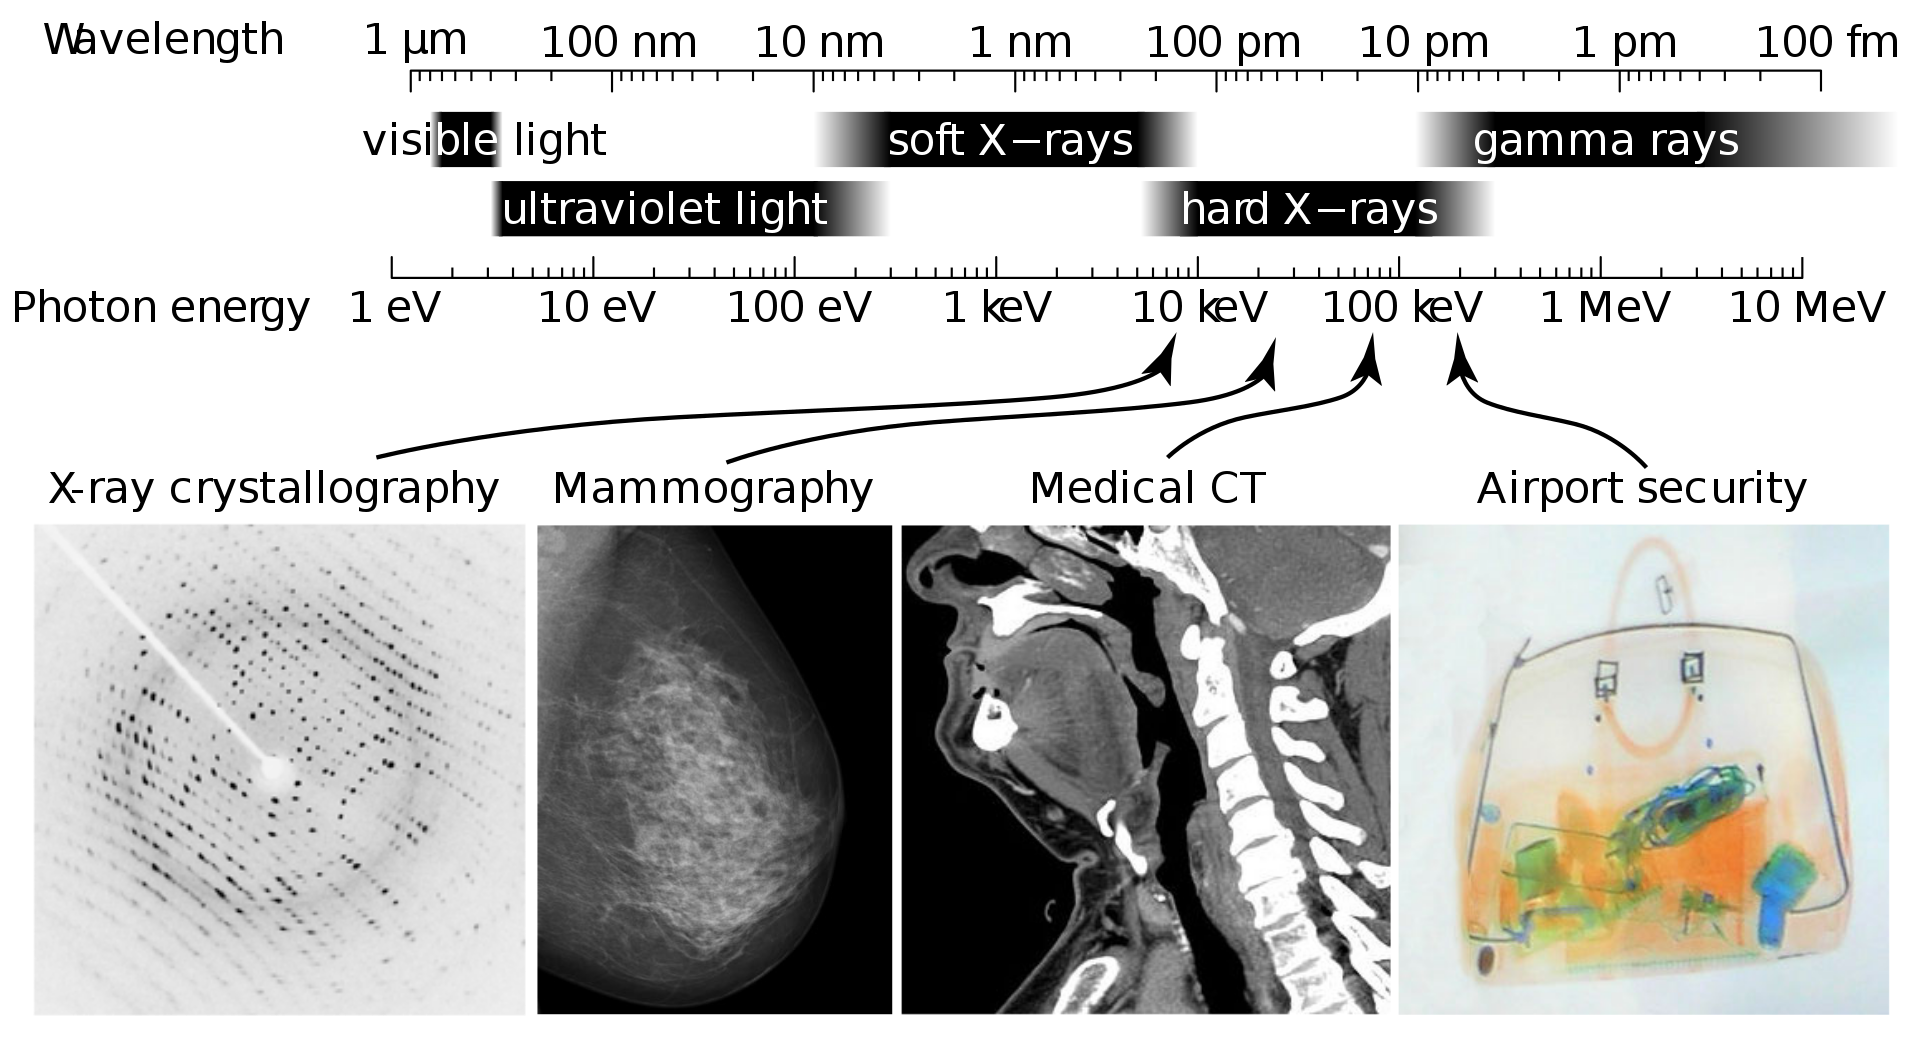
\includegraphics[width=0.8\textwidth]{XraySpectrum.png}
        \caption{X-Ray spectrum}
    \end{figure}
    \begin{itemize}
        \item X-Ray wavelengths: $6 \ \si{pm} < \lambda < 1 \ \si{nm}$
        \item Photon energy: $1,2 \ \si{keV} < E_{photon} < 0,2 \ \si{MeV}$
    \end{itemize}
\end{frame}

\begin{frame}{X-Rays generation and detection}
    \begin{columns}
        \column{0.5\textwidth}
        \underline{\textbf{X-Ray tube:}}
        \begin{itemize}
            \item Vacuum chamber
            \item Cathode
            \item Accelerating voltage
            \item Cu anode
        \end{itemize}
        \underline{\textbf{Detector:}}
        \begin{itemize}
            \item X-Ray scintillator
        \end{itemize}
        \underline{\textbf{Generated spectrum:}}
        \begin{itemize}
            \item Bremsstrahlungs-spectrum
            \item Core electron excitation
        \end{itemize}
        \column{0.5\textwidth}
        \begin{figure}
            \centering
            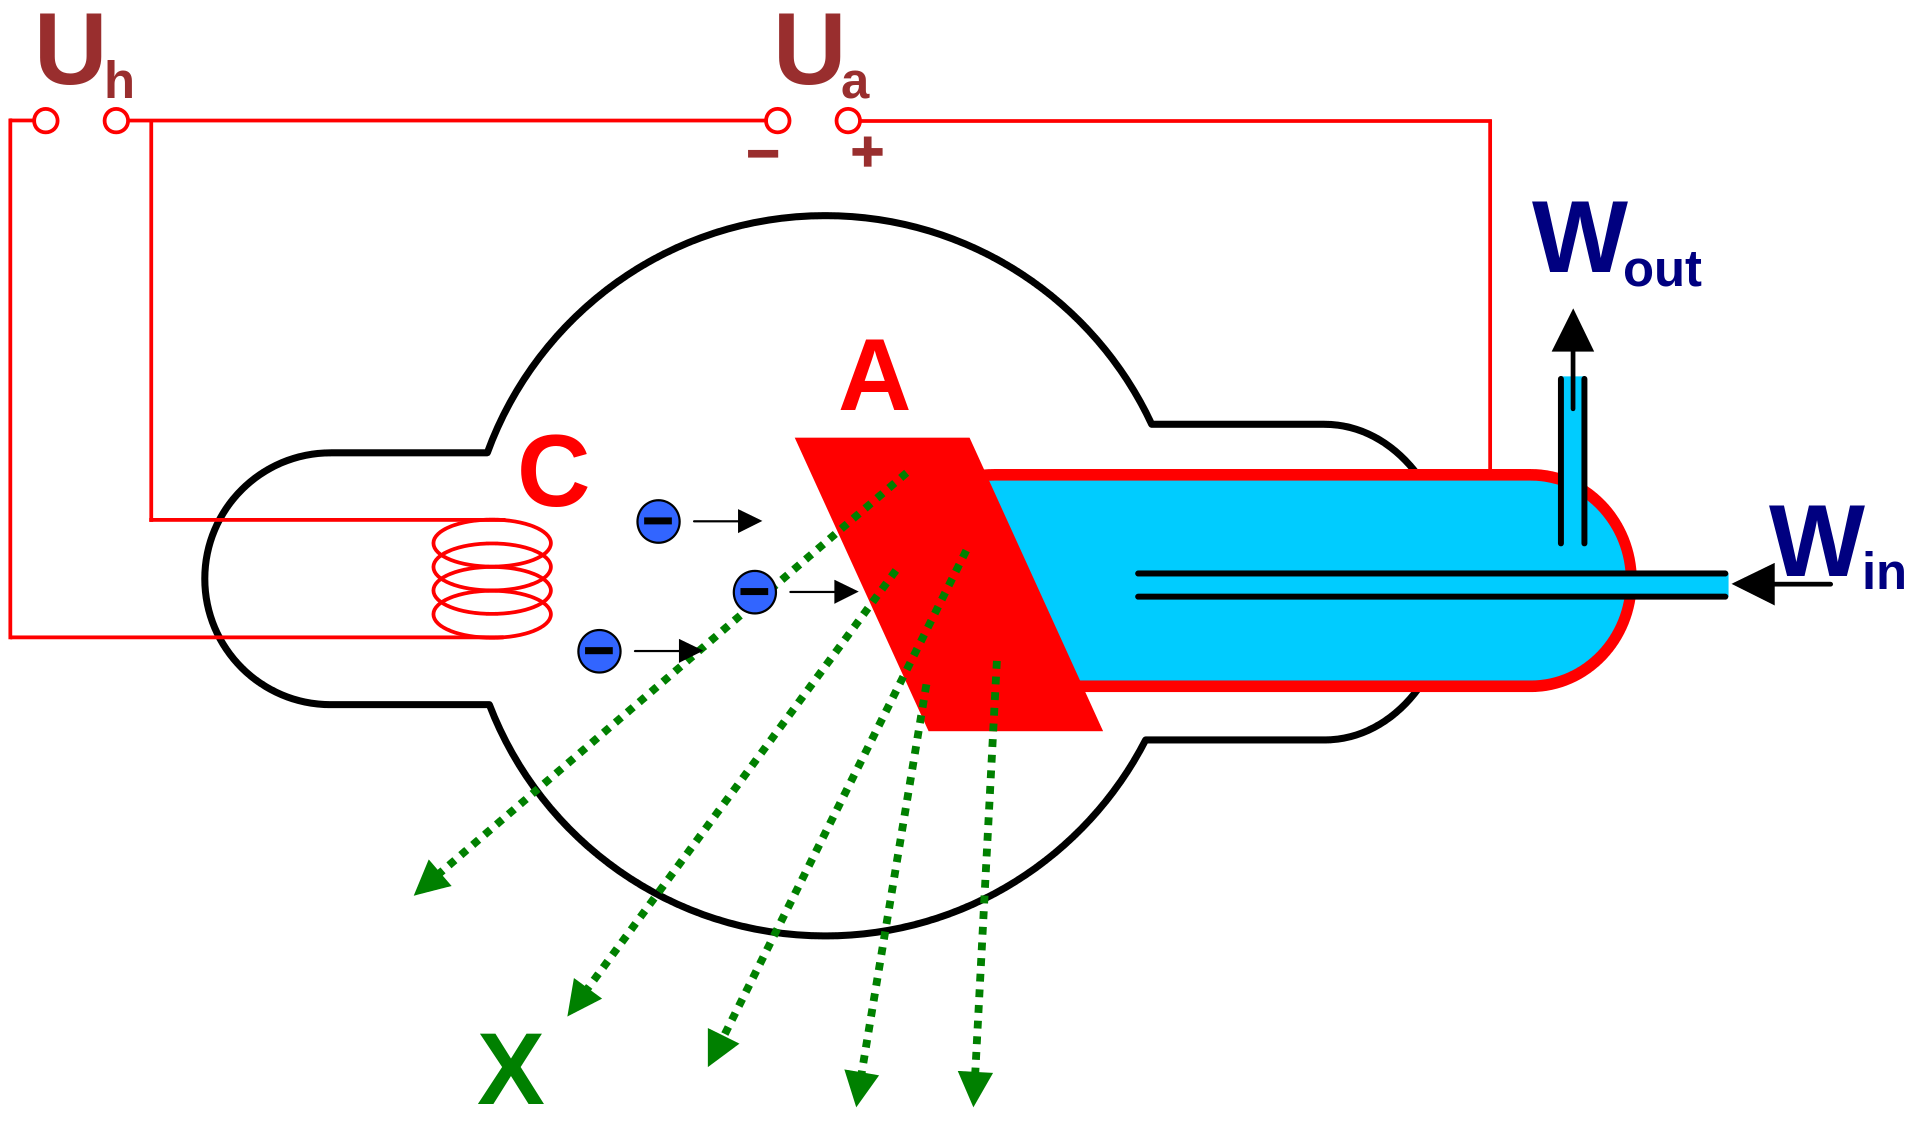
\includegraphics[width=0.8\textwidth]{xrayCathode.png}
            \caption{X-Ray tube}
        \end{figure}
        \vspace{-0.5cm}
        \begin{figure}
            \centering
            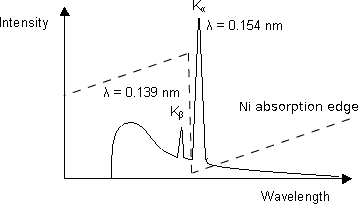
\includegraphics[width=0.8\textwidth]{CuXraySpectrum.png}
            \caption{X-Ray emission spectrum with Ni filter}
        \end{figure}
    \end{columns}    
\end{frame}

\subsection{Bragg's law}

\begin{frame}{Bragg's law}
    \begin{columns}
        \column{0.5\textwidth}
        \begin{block}{Bragg's law}
            \begin{equation*}    
                2dsin(\theta) = n \lambda
            \end{equation*}
        \begin{itemize}
            \item $d$ : lattice spacing
            \item $\theta$ : diffraction angle
            \item $\lambda$ : X-Ray wavelength
            \item $n$ : integer
        \end{itemize}
        \end{block}
        \column{0.5\textwidth}
        \begin{figure}
            \centering
            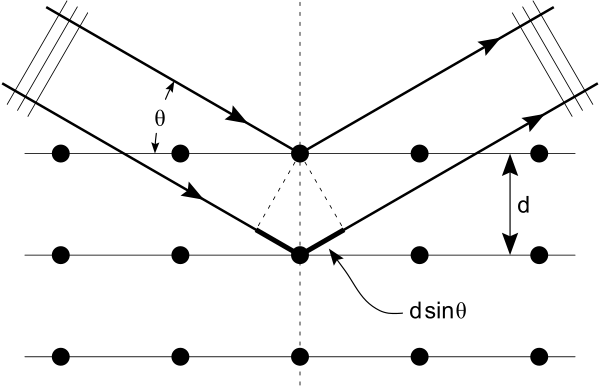
\includegraphics[width=\textwidth]{600px-Bragg_diffraction_2.svg.png}
            \caption{Illustration of Bragg's law}
            \label{fig:BraggLaw}
        \end{figure}
    \end{columns}
\end{frame}

\begin{frame}{Special case: Bragg's law for FCC crystals }
    \begin{columns}
        \column{0.5\textwidth}
        \begin{exampleblock}{Definition}
            FCC : Face-Centered-Cubic
        \end{exampleblock}
        \begin{block}{Bragg's law for FCC crystals}
            \begin{equation*}
                \frac{2a}{\sqrt{h^2 + k^2 + l^2}} \sin( \theta ) = n \lambda
                \label{eq:Bragg2}
            \end{equation*}
            \begin{itemize}
                \item $a$ : lattice constant
                \item $h,k,l$ : Miller indices
            \end{itemize}
        \end{block}
        \column{0.5\textwidth}
        \begin{figure}
            \centering
            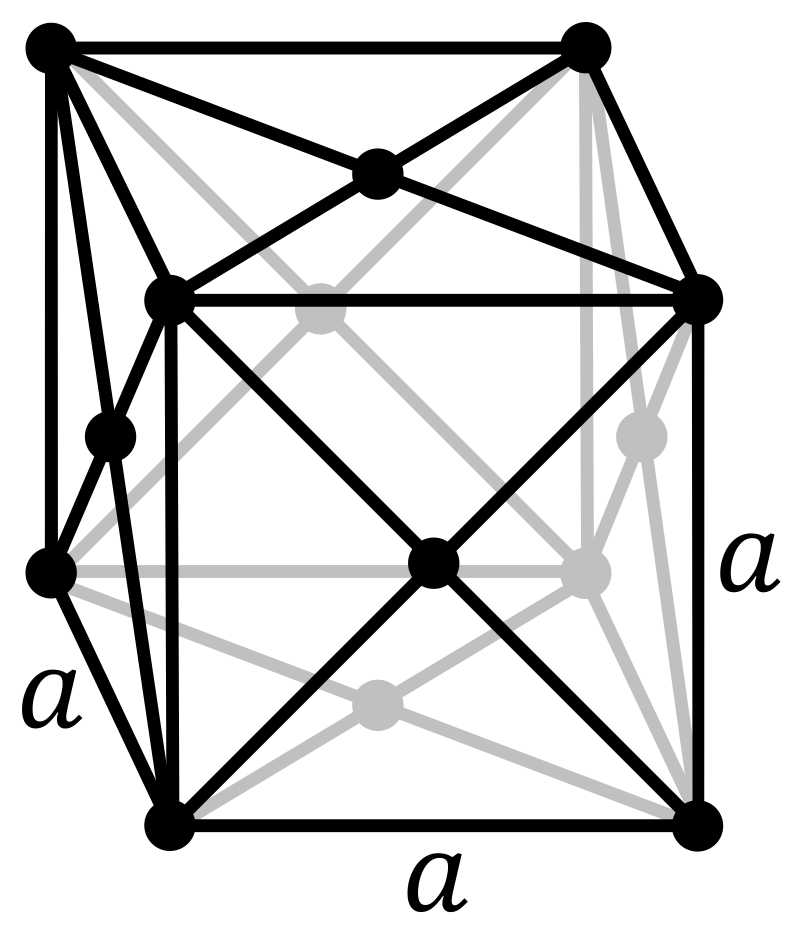
\includegraphics[width=0.5\textwidth]{800px-Cubic-face-centered.svg.png}
            \caption{Face-Centered-Cubic crystal structure}
            \label{fig:FaceCenteredCubicCrystalStructure}
        \end{figure}
    \end{columns}
    \begin{exampleblock}{Structure factor}
            \[ |F| = \frac{\text{amplitude of the wave scattered by all the atoms of a unit cell}}{\text{amplitude of the wave scattered by one electron}}\]
        \end{exampleblock}
\end{frame}

\subsection{Peak broadening}

\begin{frame}{Lorentzian and Gaussian curves}
    \begin{columns}
        \column{0.5\textwidth}
        \textbf{\underline{Key differences:}}
        \begin{itemize}
            \item Probability distributions: Cauchy and Normal
            \item Sharpness of the peak
            \item Width of the peak
        \end{itemize}
        \textbf{\underline{Ideal spectral line shape:}}
        \begin{itemize}
            \item Dirac delta
        \end{itemize}
        \column{0.5\textwidth}
        \begin{figure}
            \centering
            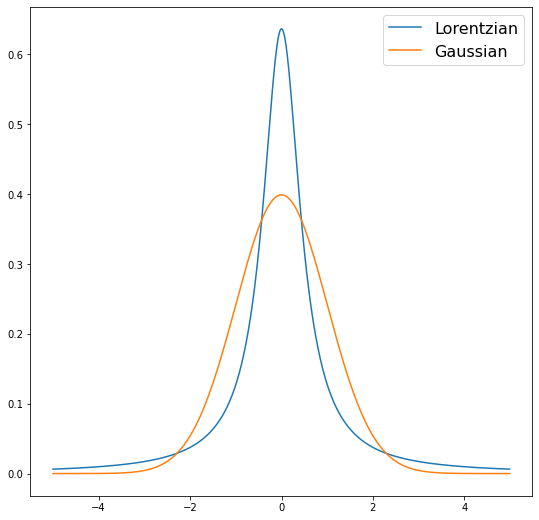
\includegraphics[width=\textwidth]{LorentzianGaussian.png}
            \caption{Normalized Lorentzian and Gaussian curves}
            \label{fig:GaussianLorentzian}
        \end{figure}
    \end{columns}
\end{frame}

\begin{frame}{Peak broadening: form and experimental sources}
    \textbf{\underline{Sources:}}
    \begin{itemize}
        \item instrumental: $\delta (2 \theta)_{inst}$
        \item crystal size: $\delta (2 \theta)_{size}$
        \item crystal strain: $\delta (2 \theta)_{strain}$
    \end{itemize}   
    \begin{block}{Lorentzian broadening}
        \begin{equation*}
            \delta(2\theta)_{total} = \delta(2\theta)_{inst} + \delta(2\theta)_{size} + \delta(2\theta)_{strain} 
        \end{equation*}
    \end{block}
    \begin{block}{Gaussian broadening}
        \begin{equation*}
            [\delta(2\theta)_{total}]^2 = [\delta(2\theta)_{inst}]^2 + [\delta(2\theta)_{size}]^2 + [\delta(2\theta)_{strain}]^2 
        \end{equation*}
    \end{block}   
\end{frame}

\section{Setup and methods}

\begin{frame}{Setup and methods}
    \begin{columns}
        \column{0.5\textwidth}
        \begin{figure}
            \centering
            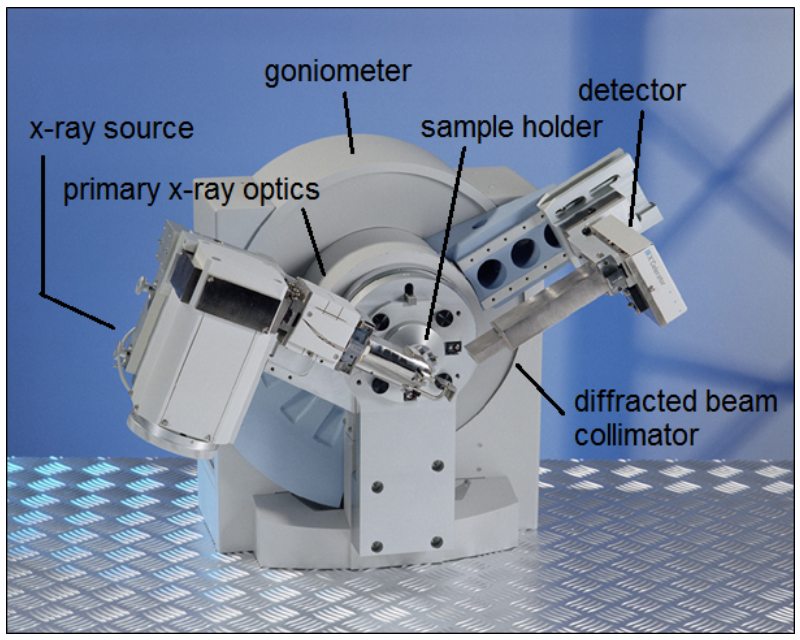
\includegraphics[width=0.7\textwidth]{XraySetup.png}
            \caption{X-Ray experiment}
        \end{figure}
        \column{0.5\textwidth}
        \begin{figure}
            \centering
            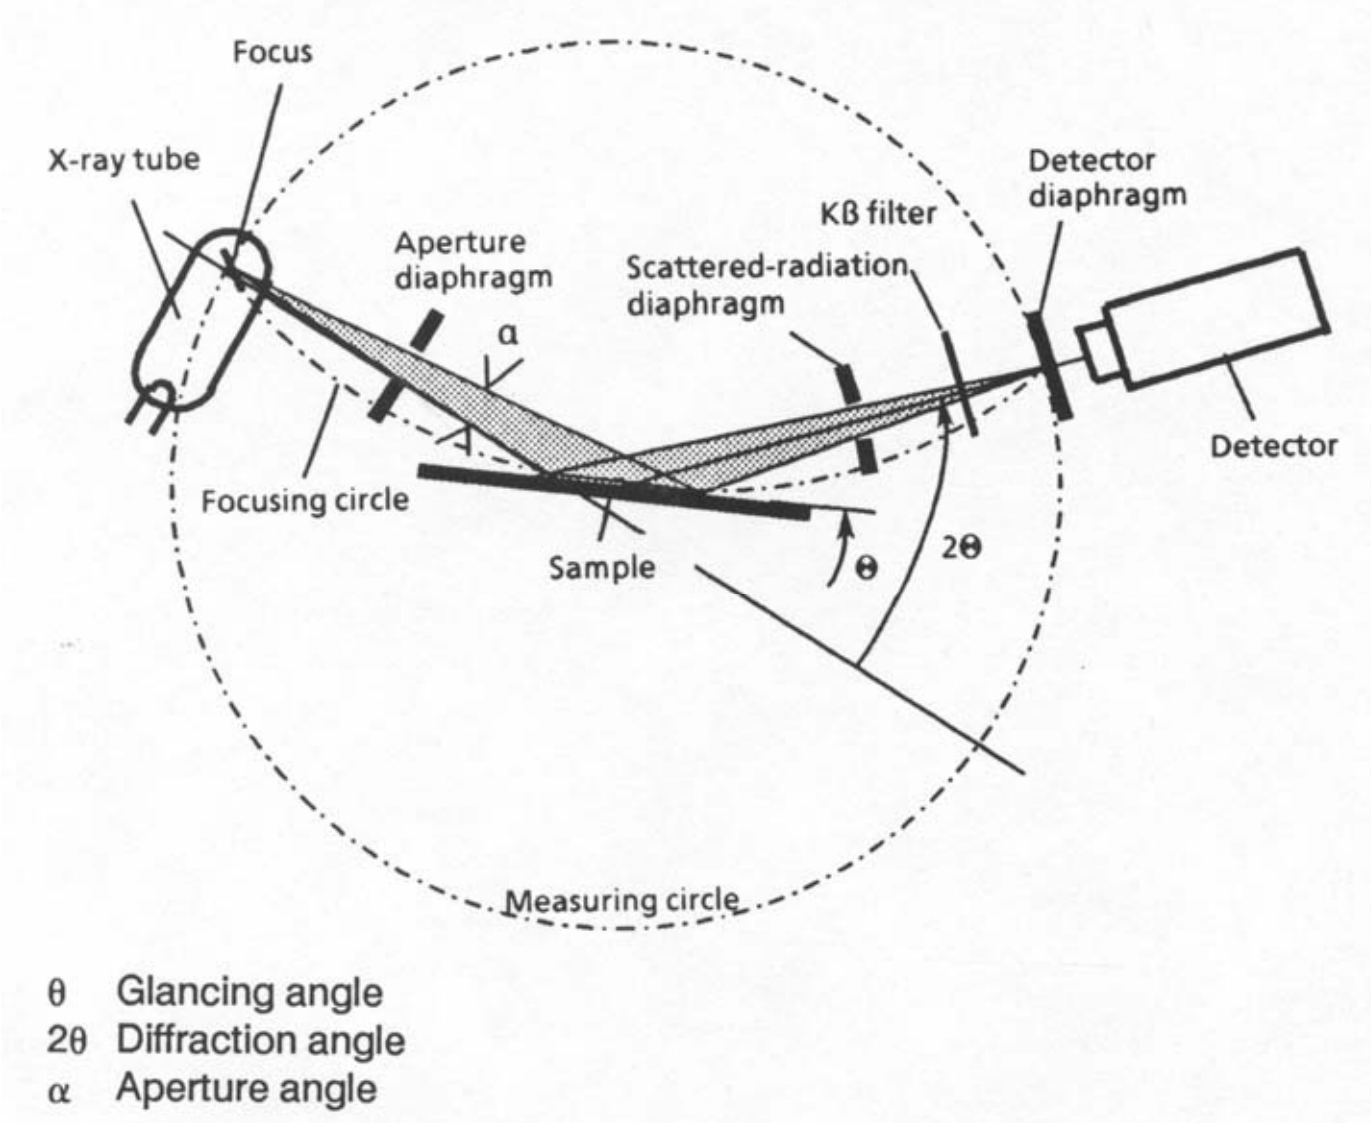
\includegraphics[width=0.7\textwidth]{XRaySetupSchematic.png}
            \caption{Schematic of the setup}
        \end{figure}
    \end{columns}
    \vspace{-0.4cm}
    \begin{exampleblock}{XRD Methods}
        \begin{table}
            \centering
            \begin{tabular}{ccc}
                ~ & $\lambda$ & $\theta$ \\ \hline
                Laue method & Variable & Fixed \\
                Rotating-crystal method & Fixed & Variable (partially) \\
                Powder method & Fixed & Variable
            \end{tabular}
        \end{table}
    \end{exampleblock}
\end{frame}

\begin{frame}{Powder method}
    \underline{\textbf{Advantage:}} For every set of planes, there will be a small percentage of crystallites that are properly oriented to diffract.
    \vspace{1cm}
    \begin{figure}
        \centering
        \begin{subfigure}[c]{0.5\textwidth}
        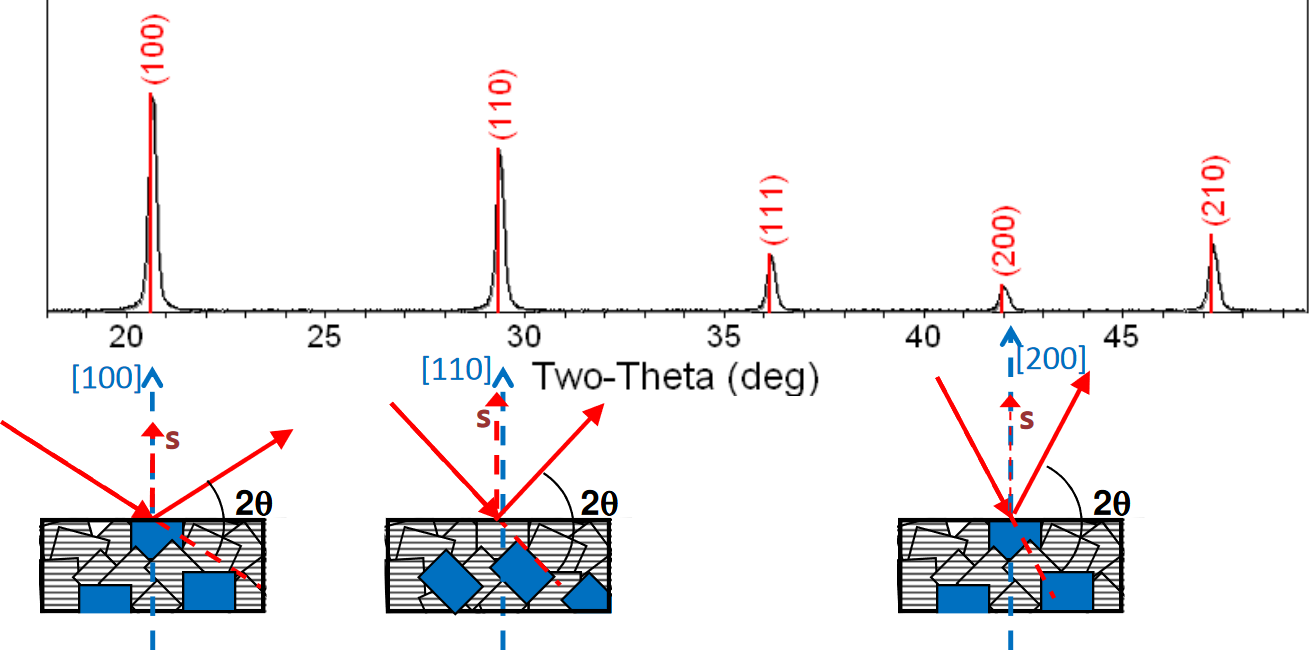
\includegraphics[width=\textwidth]{PowderMethod.png}
        \caption{Powder method illustration}
        \end{subfigure} \hfill
        \begin{subfigure}[c]{0.24\textwidth}
            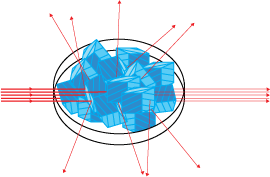
\includegraphics[width=\textwidth]{PowderMethodSimple.png}
            \caption{Scattering in multiple directions}
        \end{subfigure} \hfill
        \begin{subfigure}[c]{0.24\textwidth}
        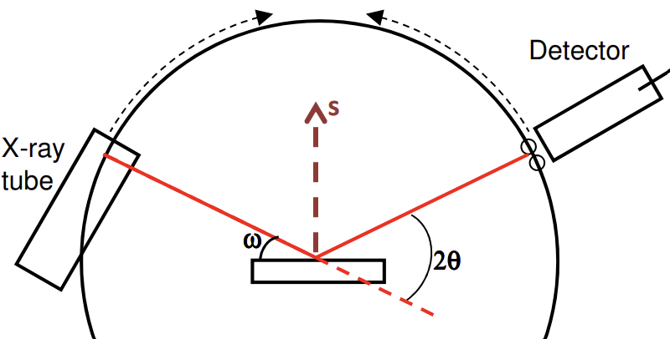
\includegraphics[width=0.9\textwidth]{BraggBrentano.png}
        \caption{Bragg-Brentano Geometry}
        \end{subfigure}
    \end{figure}
\end{frame}

\section{Results and Analysis}

\subsection{Spectra}

\begin{frame}{Experimental spectra I}
    \begin{columns}
        \column{0.5\textwidth}
        \begin{figure}
            \centering
            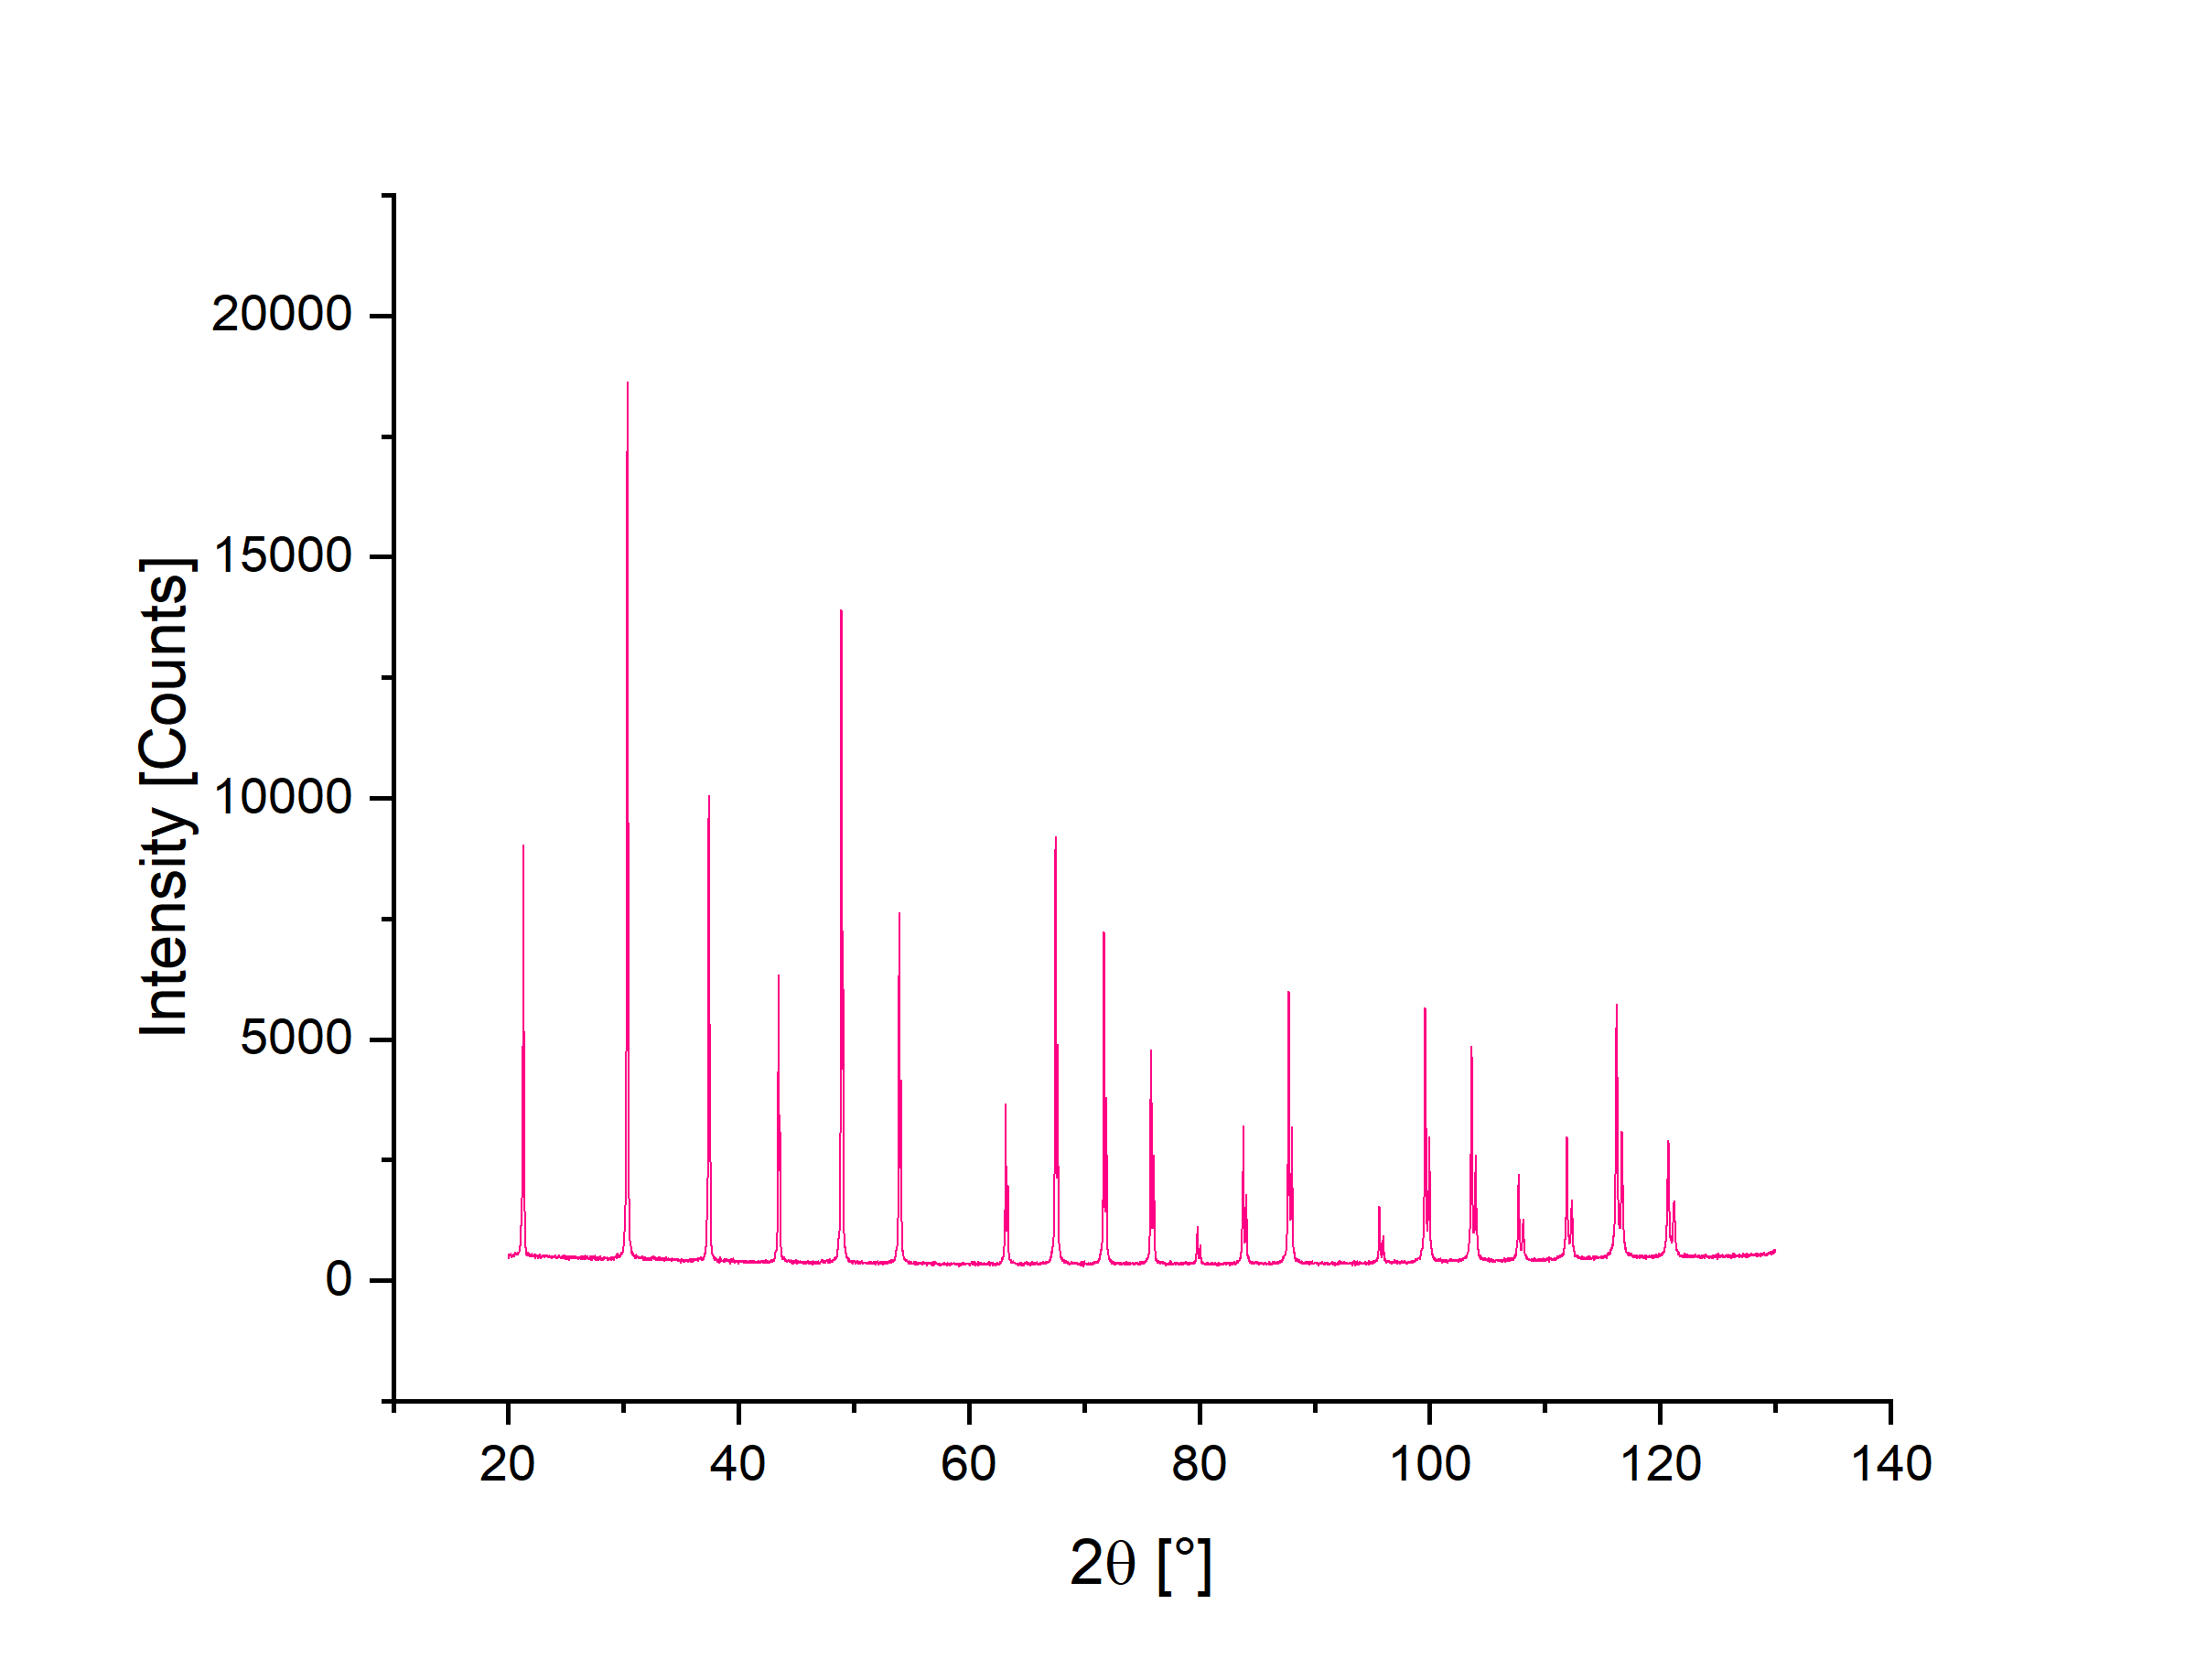
\includegraphics[width=\textwidth]{Spectrum_LaB6.png}
            \caption{Spectrum of \ce{LaB6}}
            \label{fig:SpectrumLaB6}
        \end{figure}
        \column{0.5\textwidth}
        \begin{figure}
            \centering
            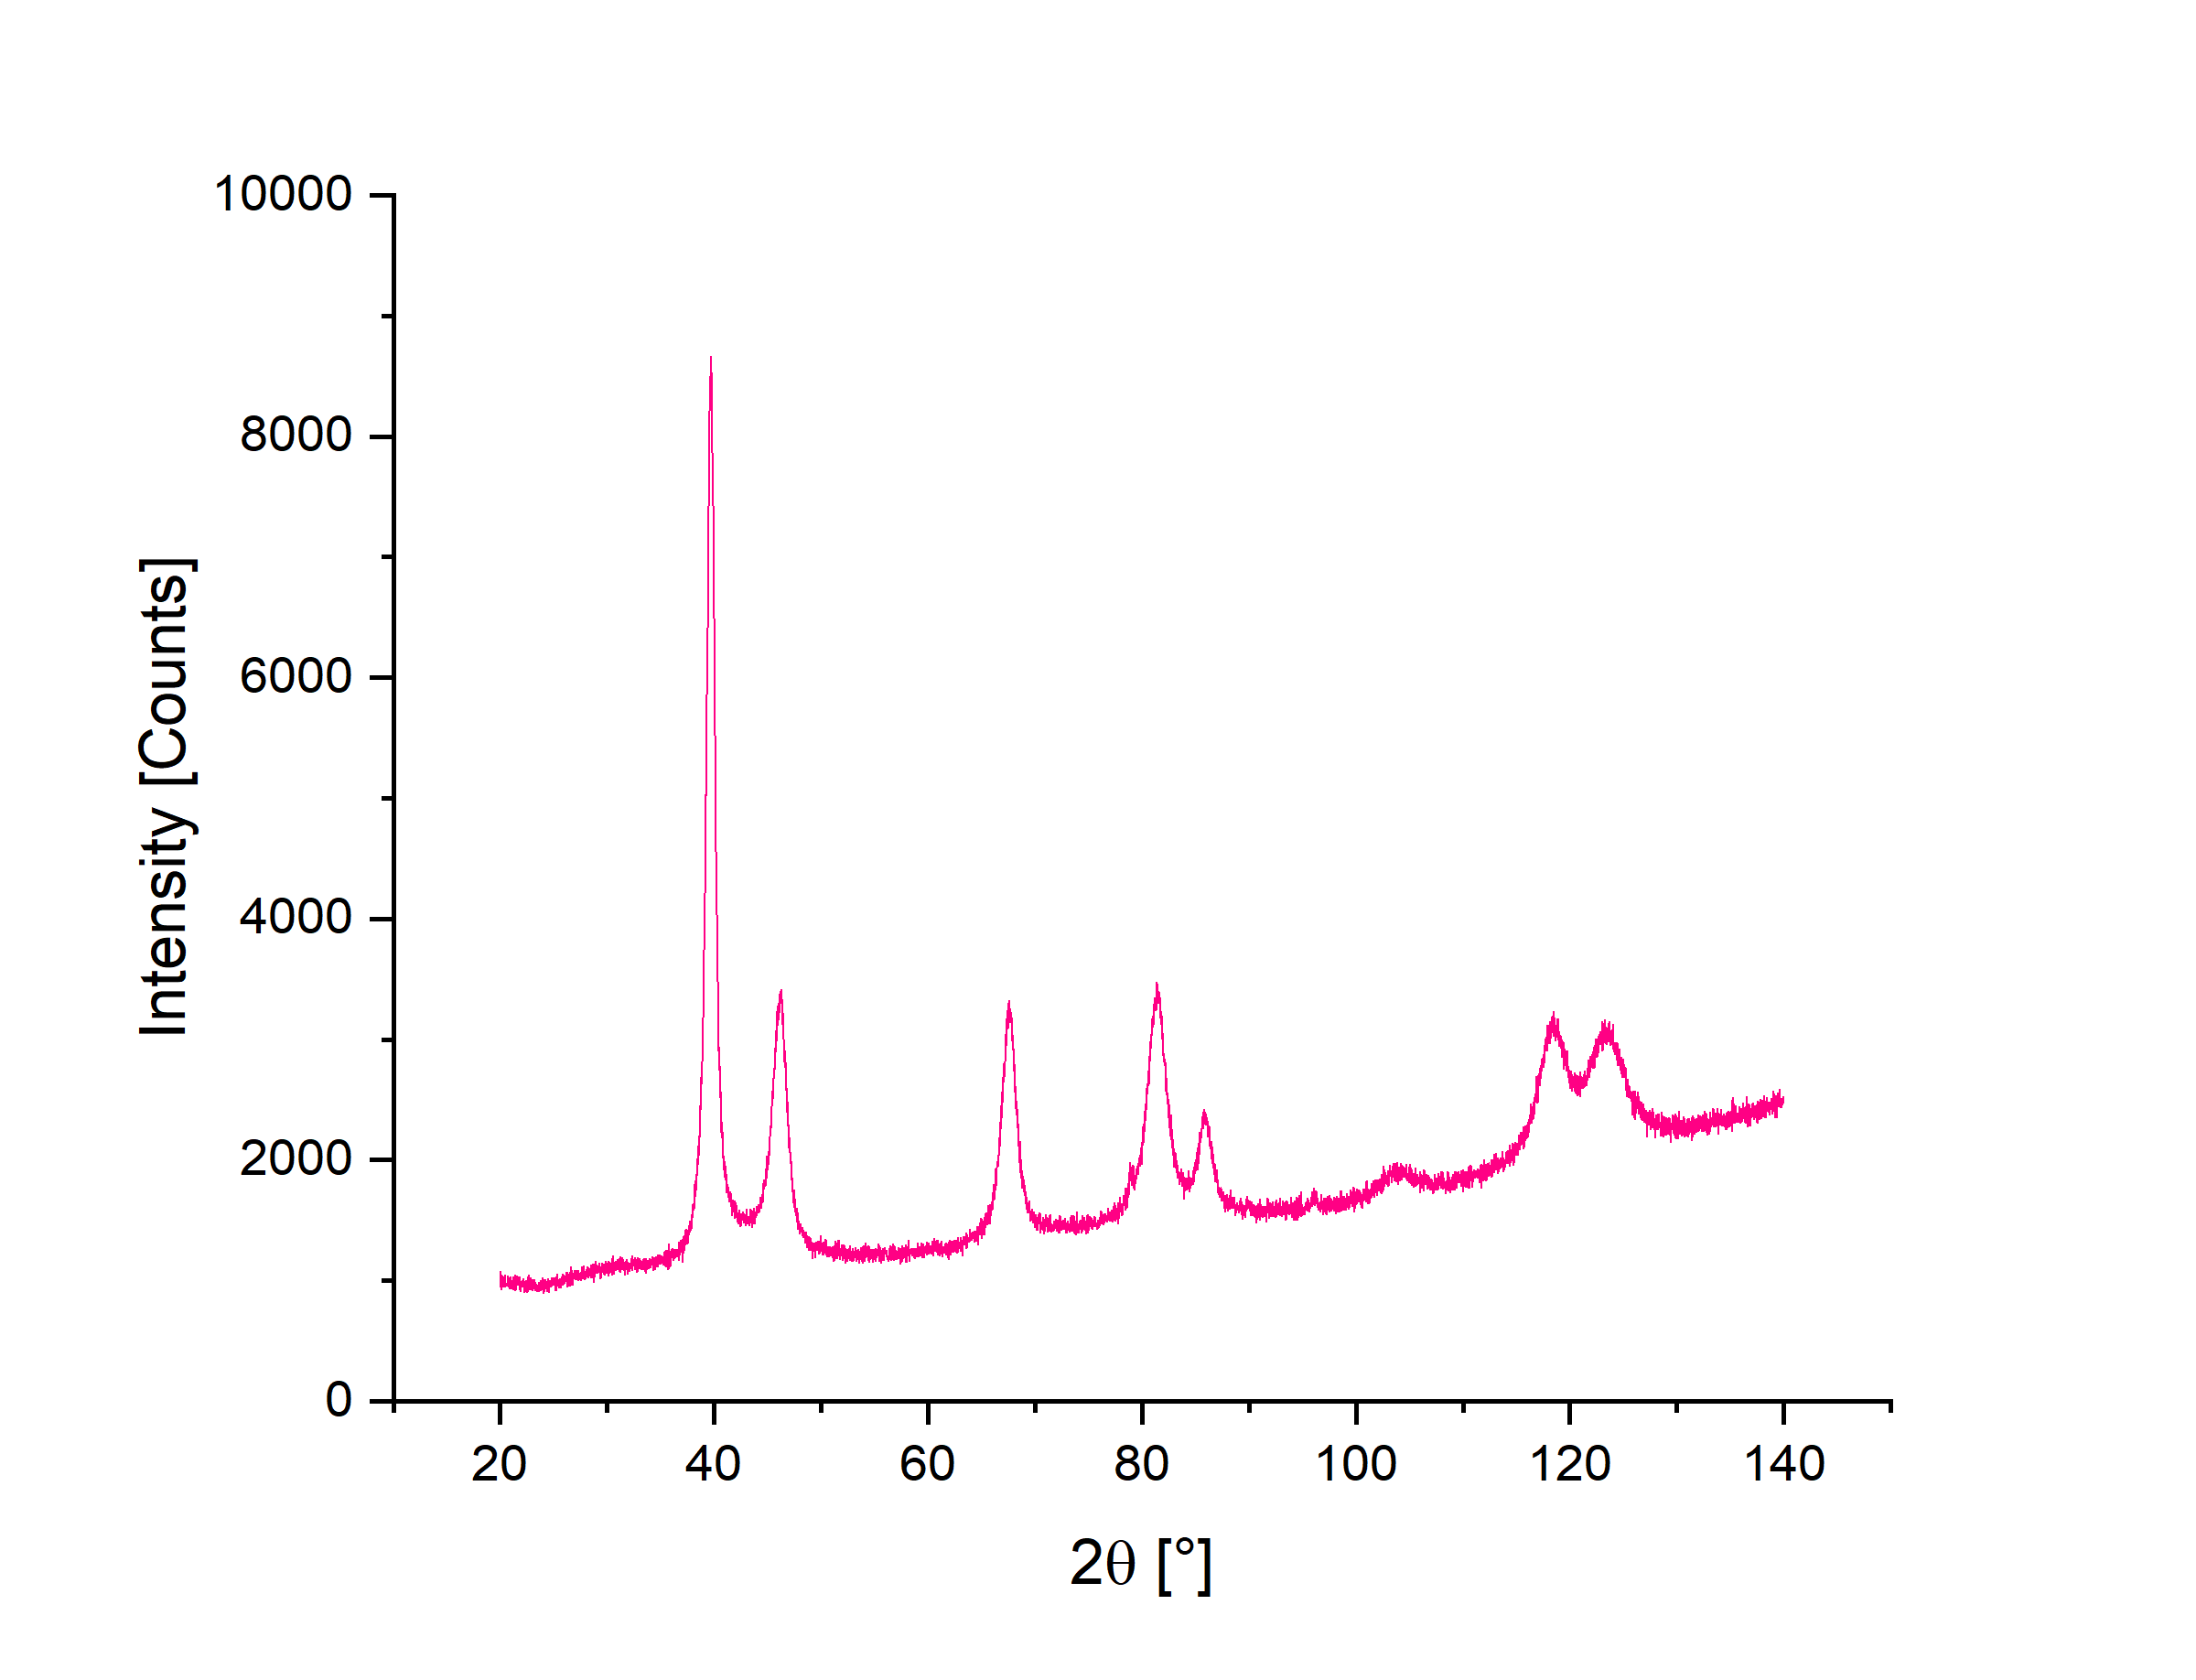
\includegraphics[width=\textwidth]{Spectrum_Pd90Au10.png}
            \caption{Spectrum of \ce{Pd90Au10}}
            \label{fig:SpectrumPd90Au10}
        \end{figure}
    \end{columns}
\end{frame}

\begin{frame}{Experimental spectra II}
    \begin{columns}
        \column{0.5\textwidth}
        \begin{figure}
            \centering
            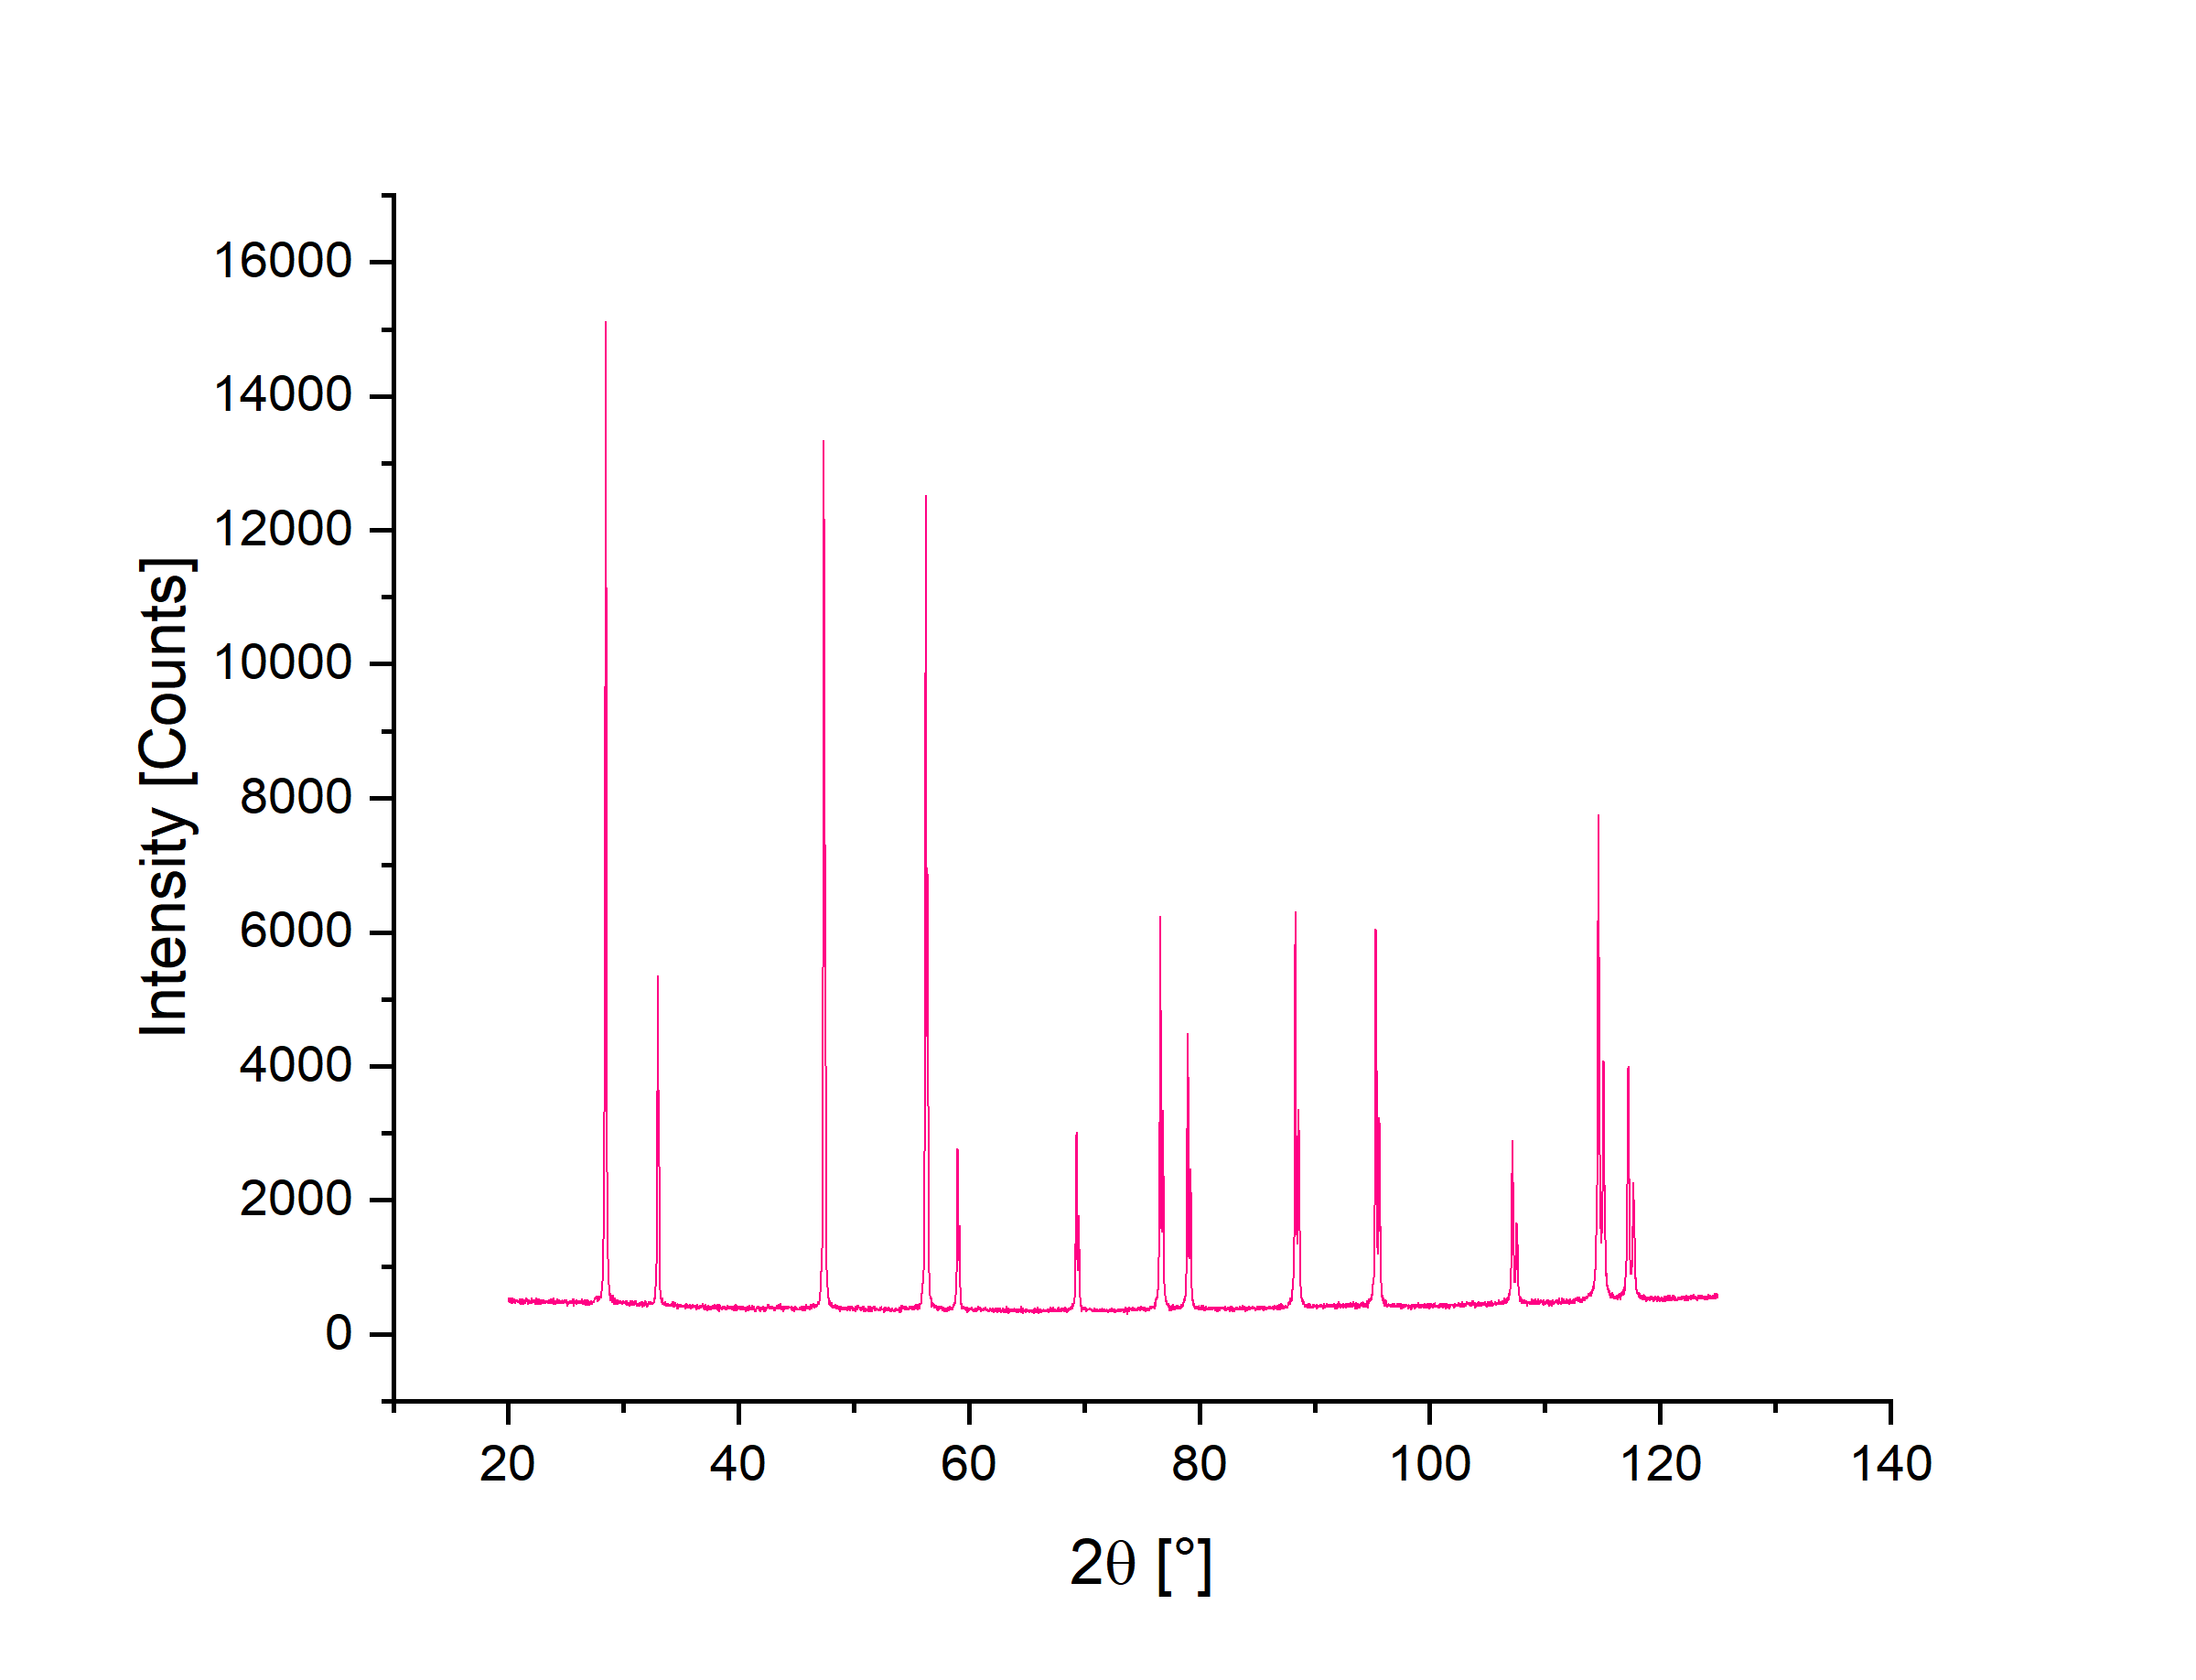
\includegraphics[width=\textwidth]{Spectrum_CeO2_1.png}
            \caption{Spectrum of micro-crystalline \ce{CeO2}}
            \label{fig:SpectrumCeO2_1}
        \end{figure}
        \column{0.5\textwidth}
        \begin{figure}
            \centering
            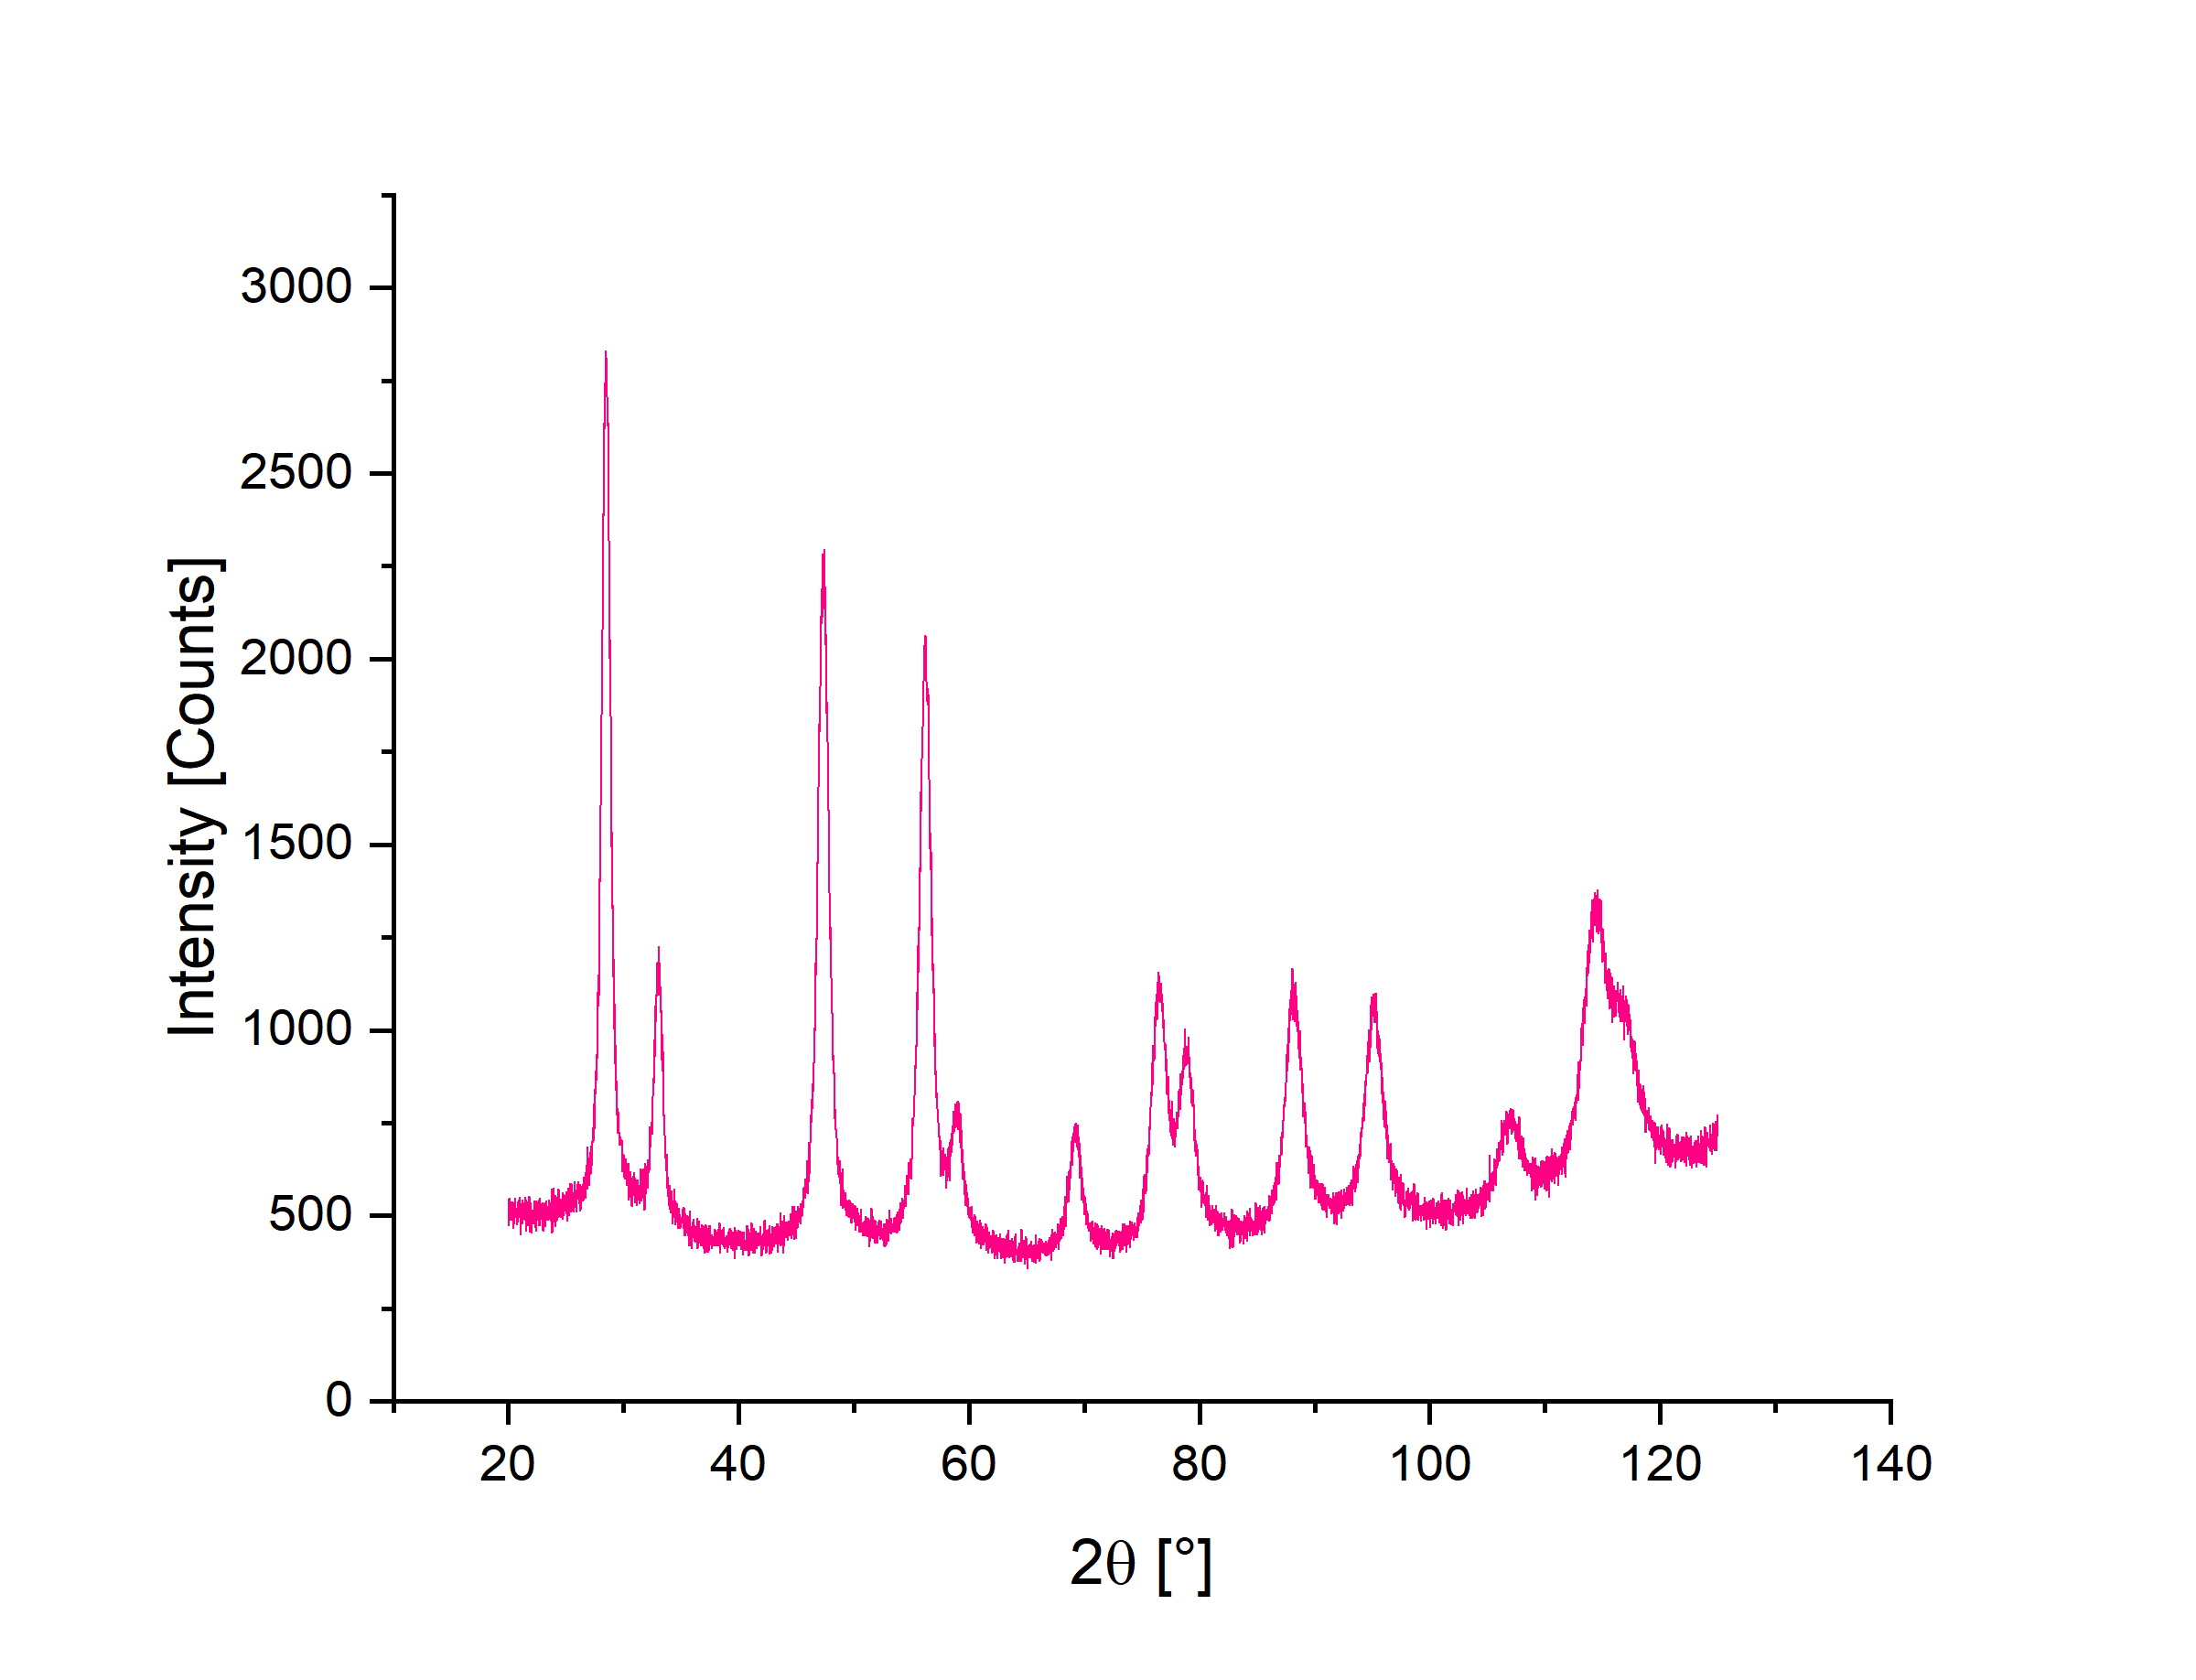
\includegraphics[width=\textwidth]{Spectrum_CeO2_2.png}
            \caption{Spectrum of nano-crystalline \ce{CeO2}}
            \label{fig:SpectrumCeO2_2}
        \end{figure}
    \end{columns}
\end{frame}

\subsection{Lattice constant}

\begin{frame}{Computation of the lattice constant}
    \onslide<1->\begin{alertblock}{Lattice constant}
        \begin{equation*}
            a = \frac{n \lambda}{2 \sin(\theta)}\sqrt{h^2 + k^2 + l^2}
        \end{equation*}
    \end{alertblock}
    \onslide<2->\begin{exampleblock}{Lattice constant fit equation}
        \begin{equation*}
            a = a_0 - \left( a_0 \frac{\tilde{d}}{r} \right) \frac{\cos^2(\theta)}{\sin(\theta)}
        \end{equation*}
        \begin{itemize}
            \item $a_0$ : true lattice constant
            \item $\tilde{d}$ : sample displacement
            \item $r$ : diffractometer radius
        \end{itemize}
    \end{exampleblock}
\end{frame}

\begin{frame}{Lattice constants}
    \vspace{-1.2cm}
    \onslide<1-> \begin{columns}
        \column{0.33\textwidth}
        \begin{figure}
            \centering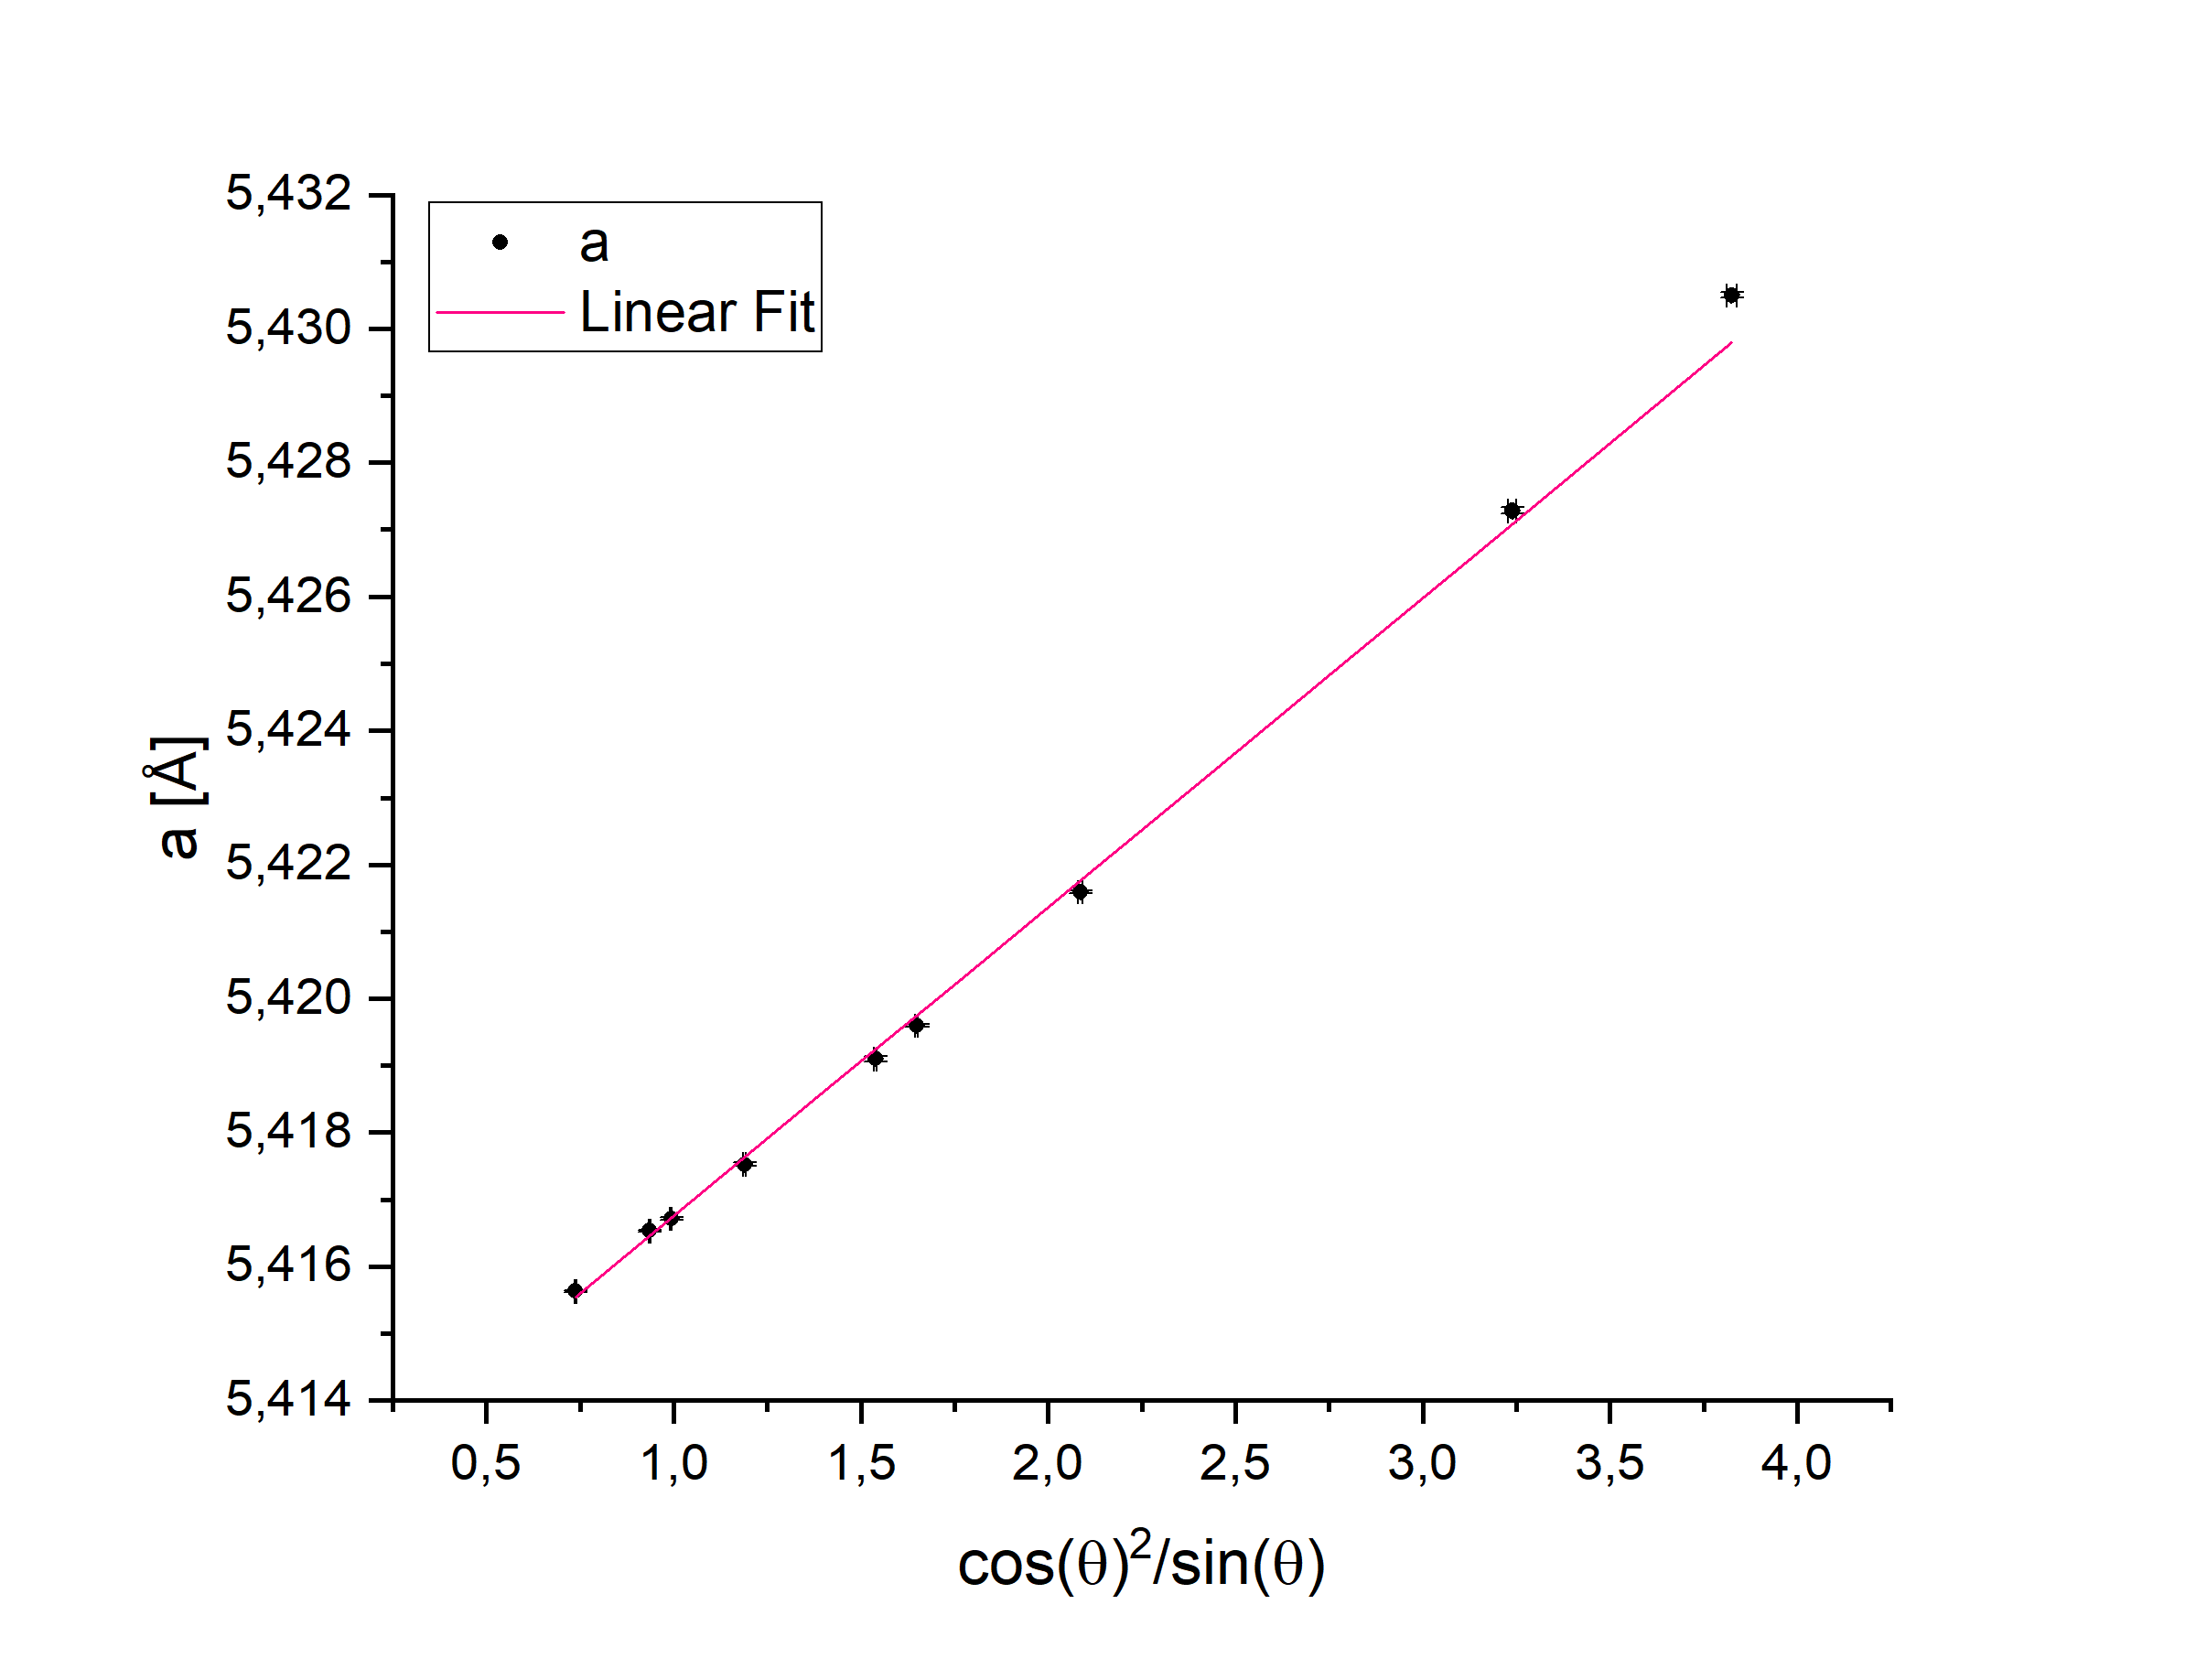
\includegraphics[width=1.1\textwidth]{LatticeConstant_CeO2_1.png}
            \caption{Micro-crystalline \ce{CeO2}}
        \end{figure}
        \column{0.33\textwidth}
        \begin{figure}
            \centering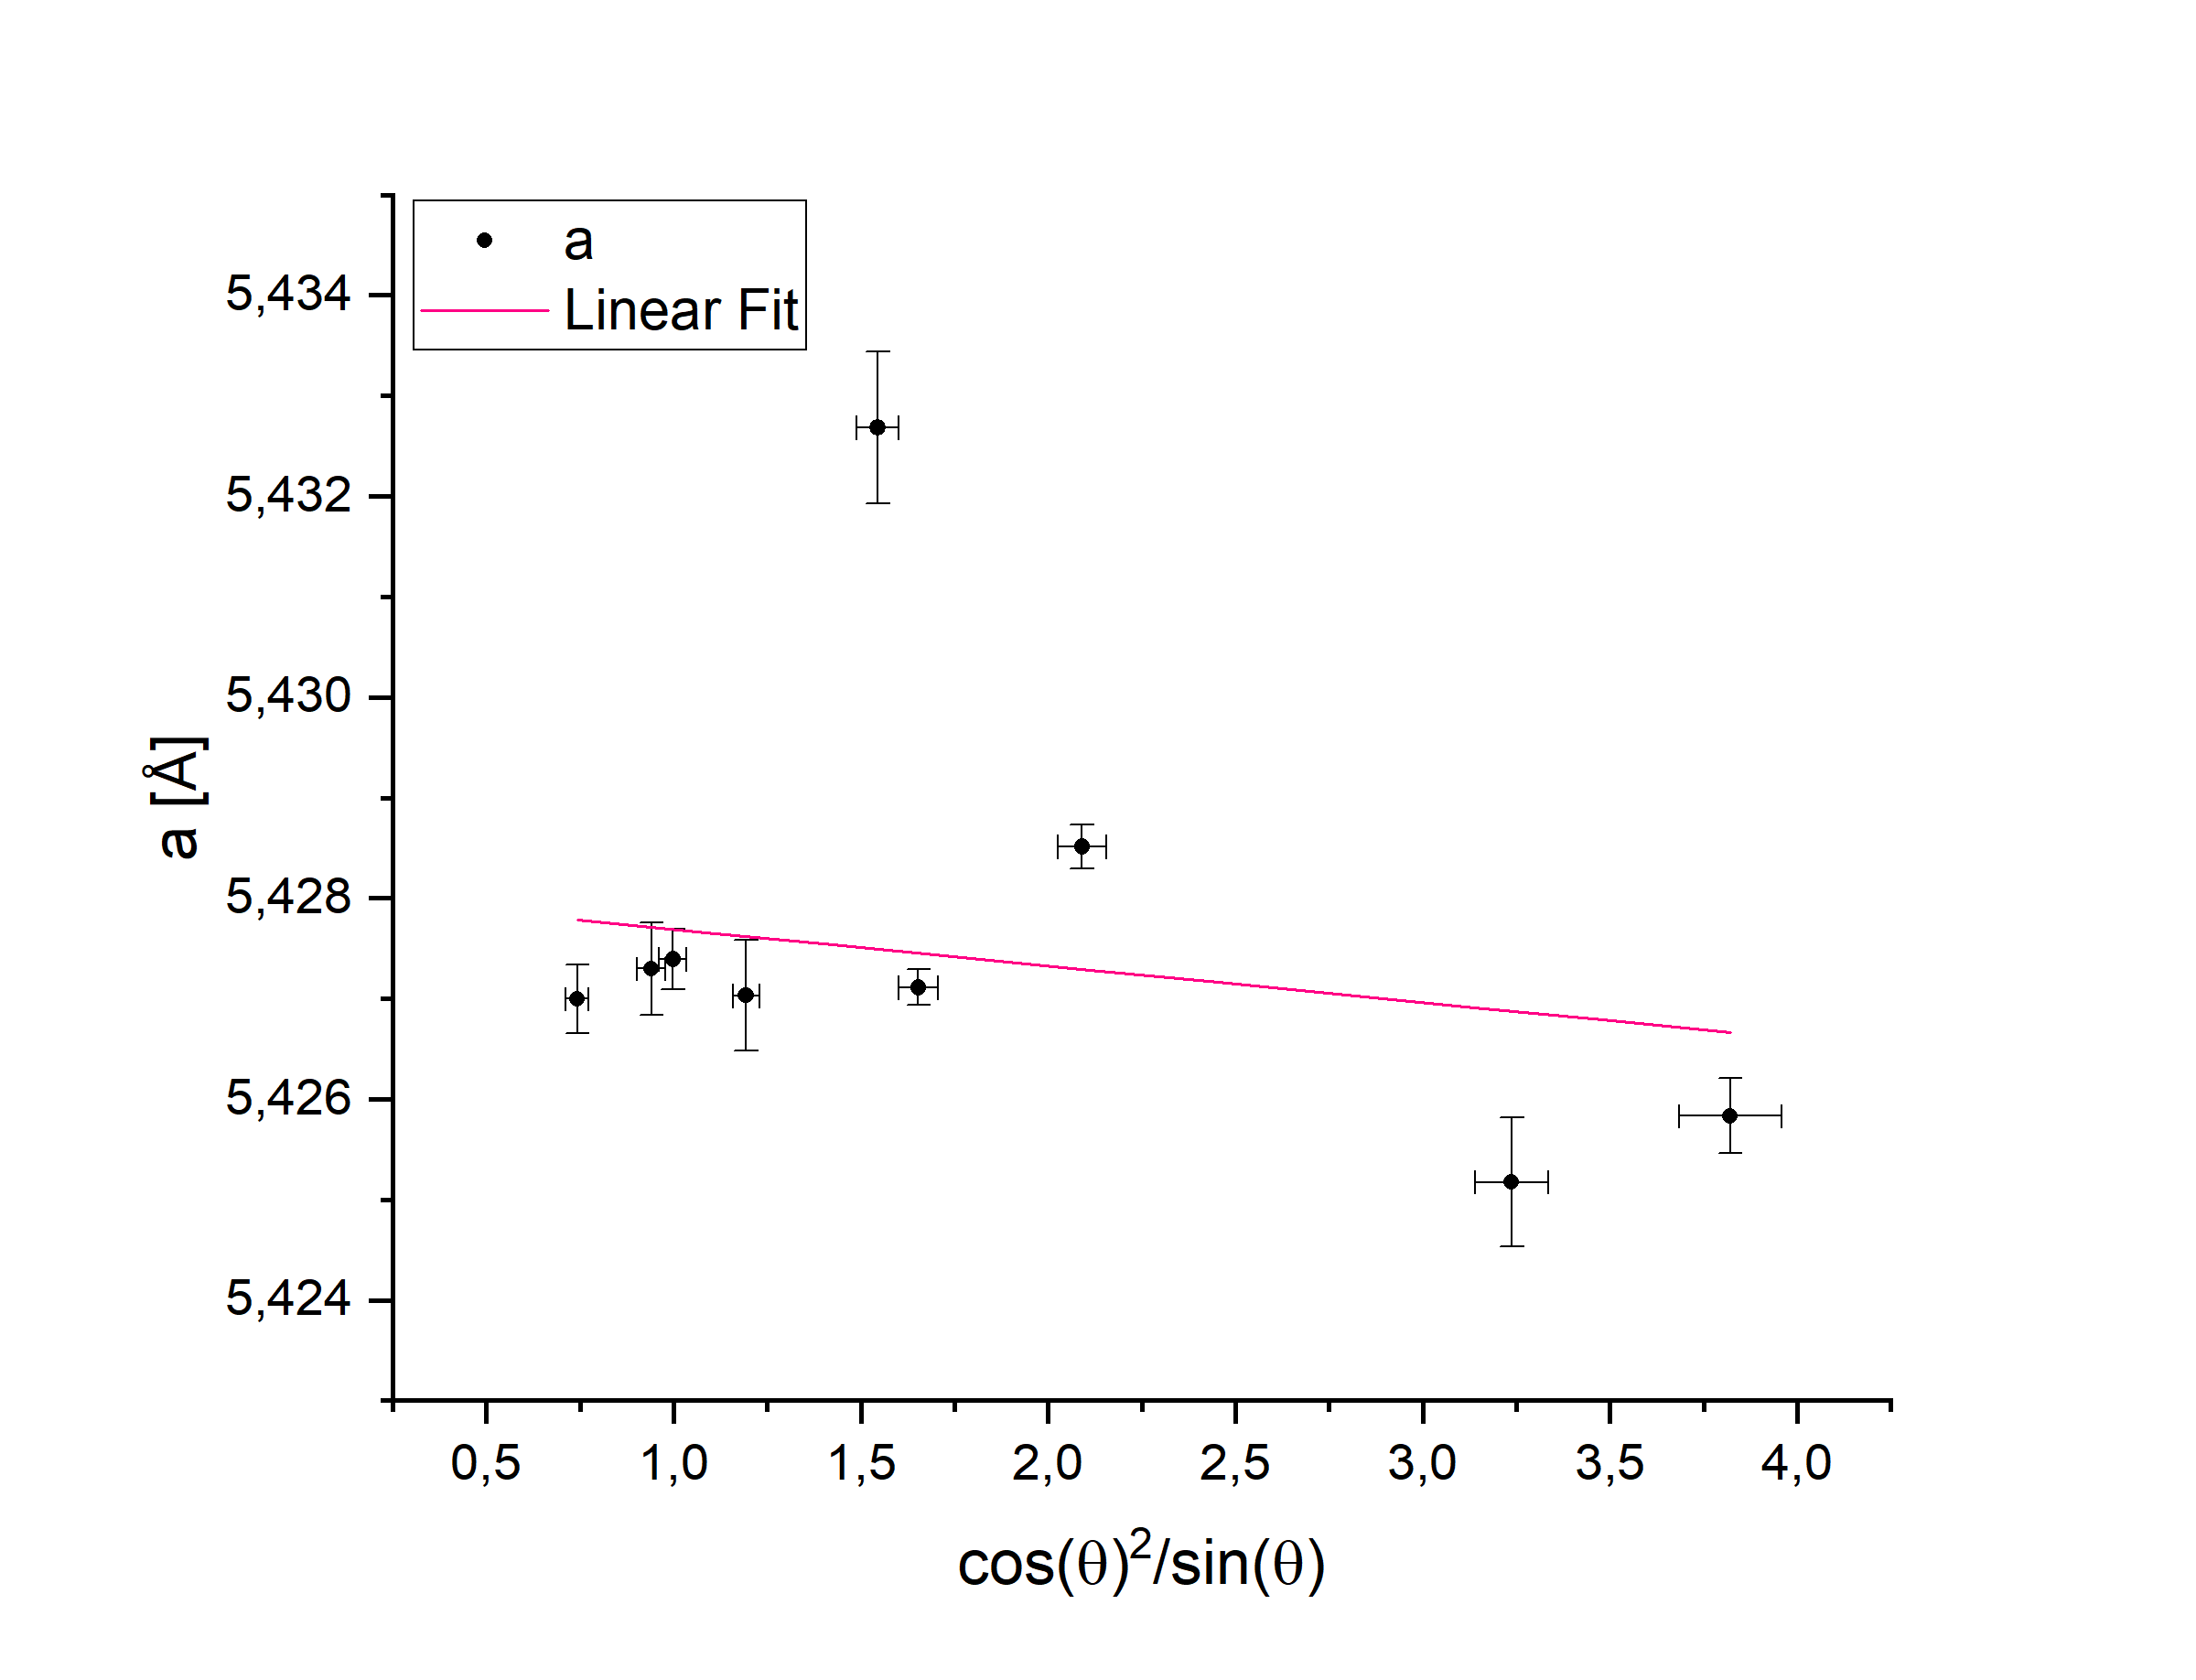
\includegraphics[width=1.1\textwidth]{LatticeConstant_CeO2_2.png}
            \caption{Nano-crystalline \ce{CeO2}}
        \end{figure}
        \column{0.33\textwidth}
        \begin{figure}
            \centering
            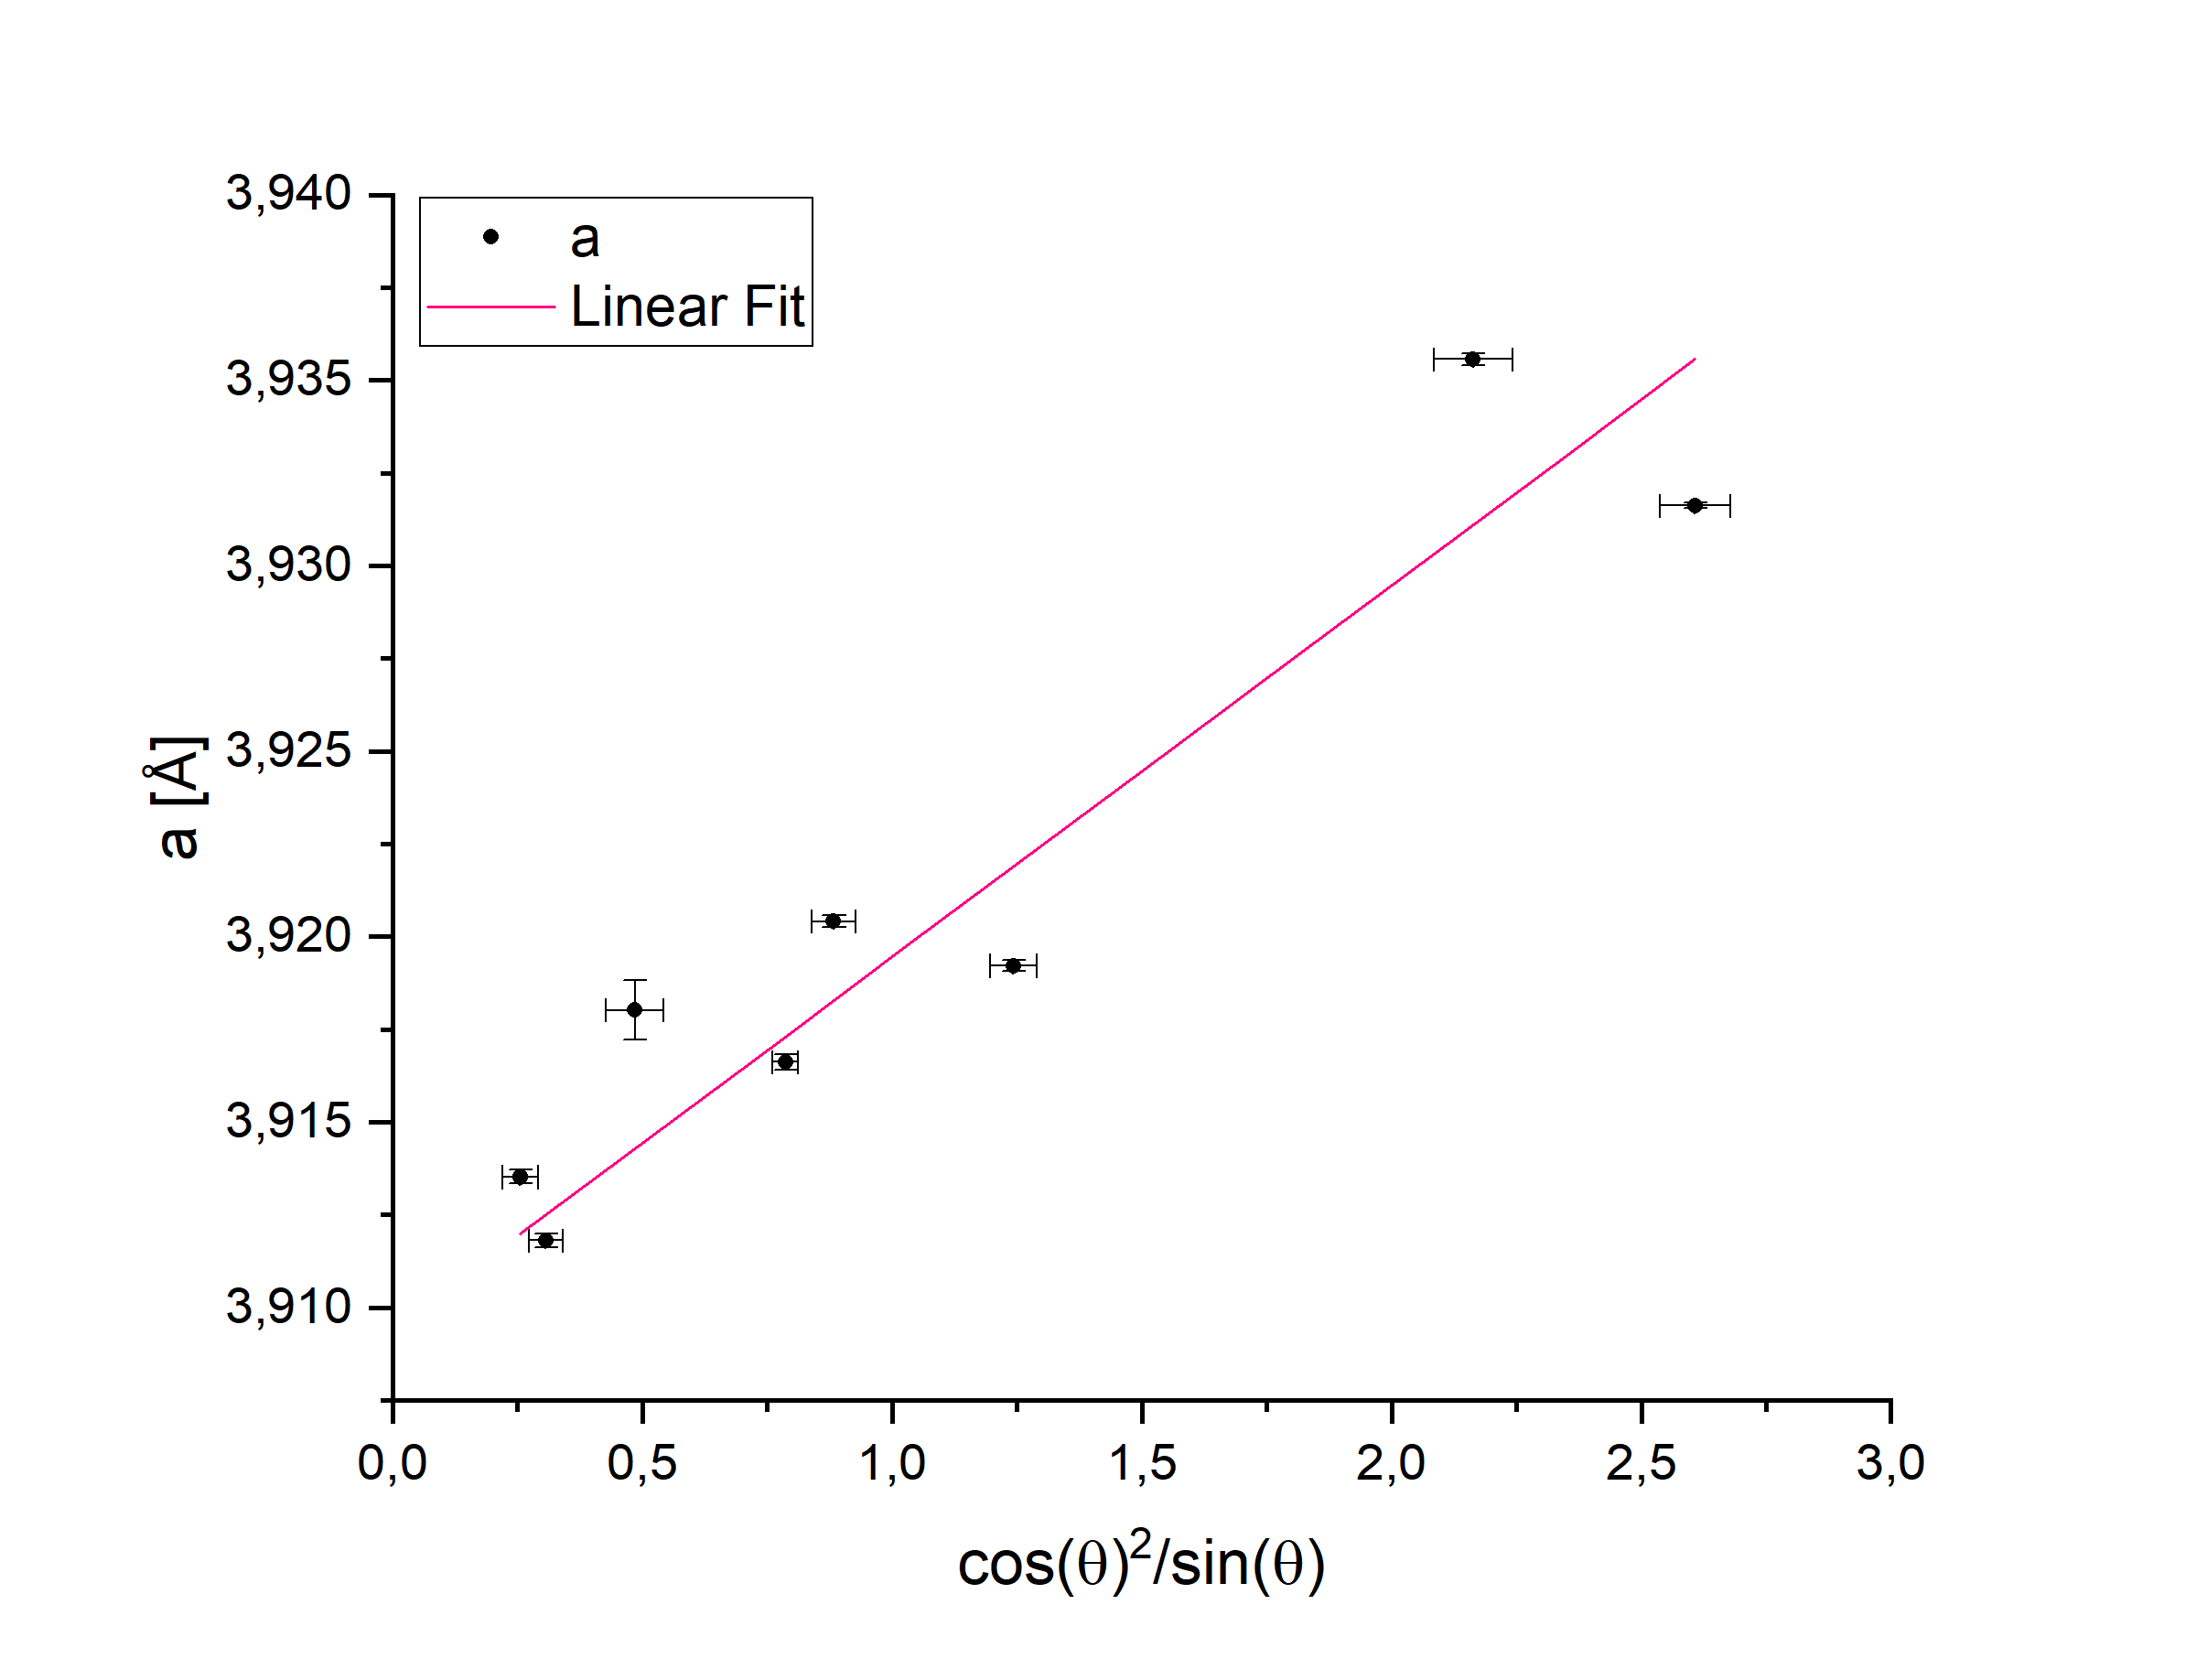
\includegraphics[width=1.1\textwidth]{LatticeConstant_Pd90Au10.png}
            \caption{\ce{Pd90Au10}}
        \end{figure}
    \end{columns}
    \vspace{-0.5cm}
    \onslide<2-> \begin{block}{Lattice constant values}
        \begin{align*}
            a_0^{\ce{CeO2},1} &= (5,4122 \pm 0,0002) \ \si{\angstrom} \\
            a_0^{\ce{CeO2},2} &= (5,4282 \pm 0,0009) \ \si{\angstrom} \\
            a_0^{\ce{Pd90Au10}} &= (3,9111 \pm 0,0022) \ \si{\angstrom}
        \end{align*}
    \end{block}
\end{frame}

\begin{frame}{Instrumental broadening}
    \begin{columns}
        \column{0.5\textwidth}
        \begin{figure}
            \centering
            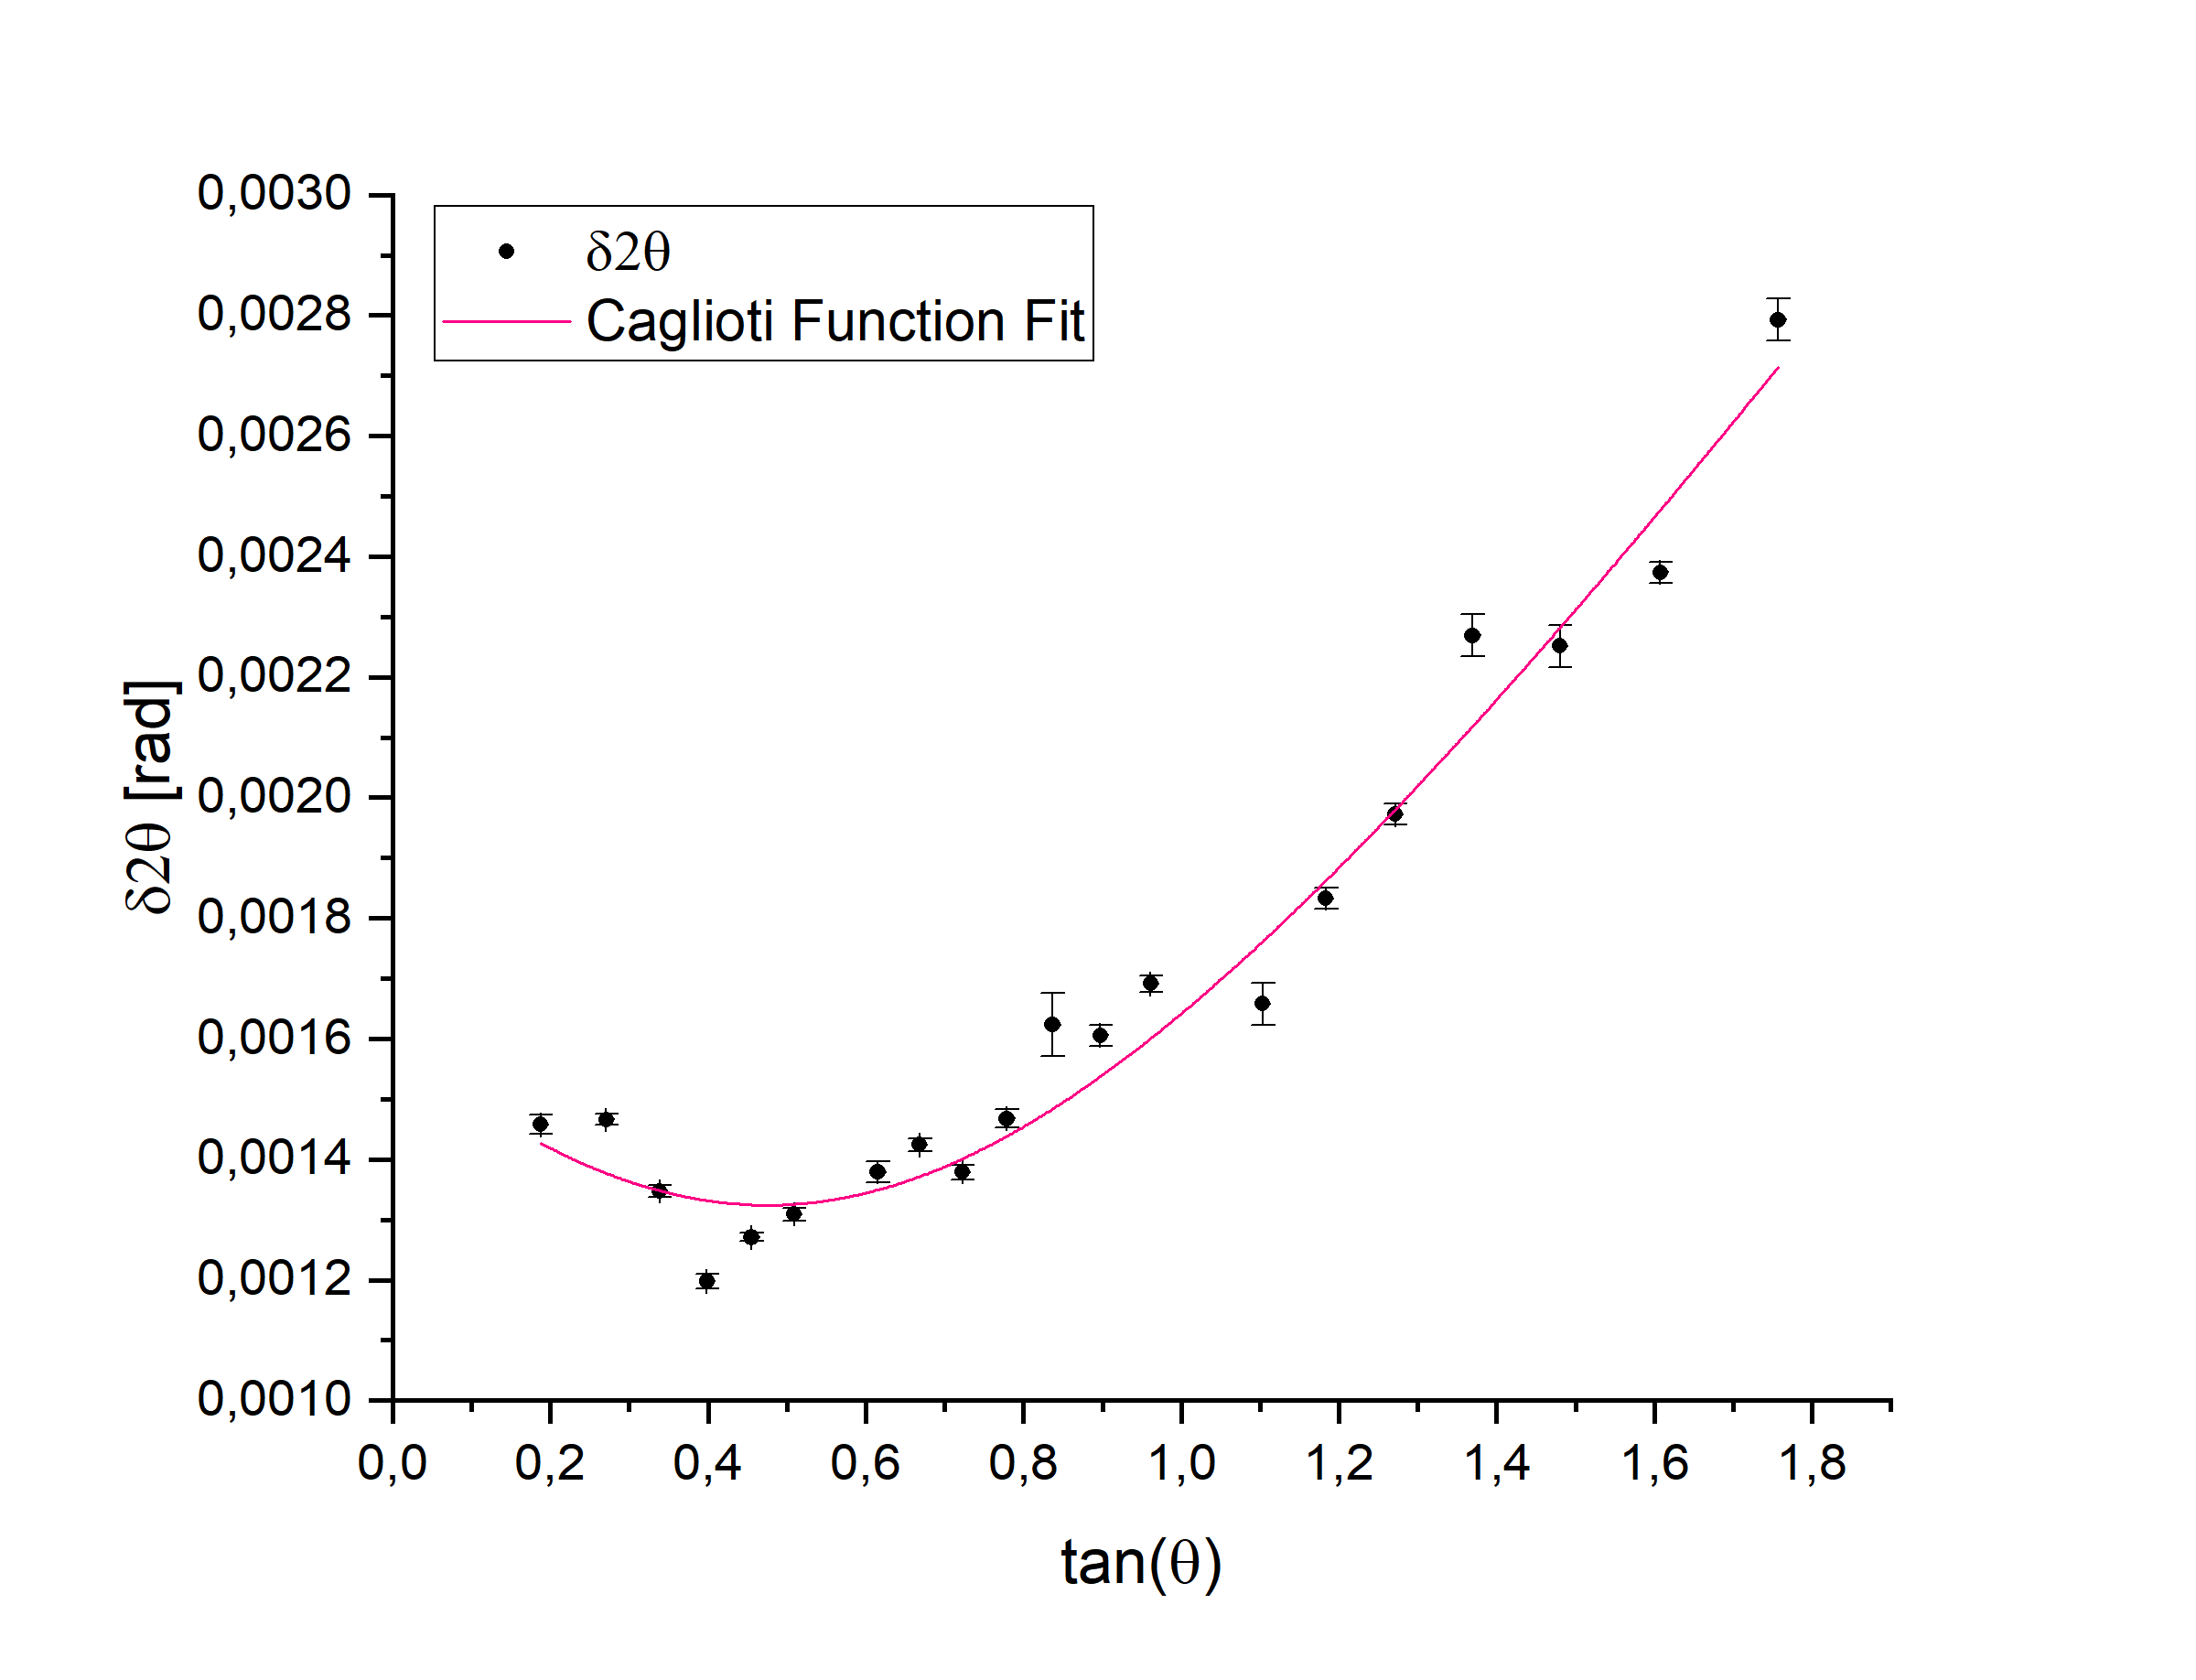
\includegraphics[width=\textwidth]{CagliotiFit.png}
            \caption{Caglioti function fit}
            \label{fig:CagliotiFunctionFit}
        \end{figure}
        \column{0.5\textwidth}
        \begin{exampleblock}{Caglioti function}
            \begin{equation*}
                f(\theta) = \sqrt{A + B\tan(\theta) + C\tan^2(\theta)}
            \end{equation*}
        \end{exampleblock}
        \begin{block}{Coefficient values}
                \begin{align*}
                    &A = ( 2,53\pm 0,21 ) \cdot 10^{-6} \ \text{rad}^2 \\
                    &B = (-3,25 \pm 0,61 ) \cdot 10^{-6} \ \text{rad}^2 \\
                    &C = ( 3,42 \pm 0,39 ) \cdot 10^{-6} \ \text{rad}^2
                \end{align*}
        \end{block}
    \end{columns}
\end{frame}

\subsection{Crystallite size and strain}

\begin{frame}{Size and strain}
    \begin{columns}
        \column{0.45\textwidth}
        \begin{figure}
            \centering
            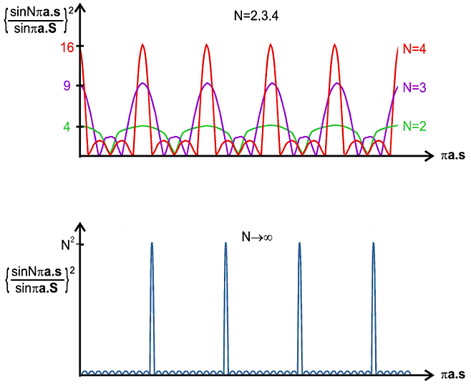
\includegraphics[width=0.8\textwidth]{CrystalliteSize.png}
            \caption{Peak intensity as function of lattice points}
        \end{figure}
        \vspace{-0.5cm}
        \begin{exampleblock}{Scherrer equation}
        \begin{equation*}
            D = \frac{6 \lambda}{ 5 \delta(2\theta) \cos(\theta)}
        \end{equation*}
        \end{exampleblock}
        \column{0.5\textwidth}
        \begin{figure}
            \centering
            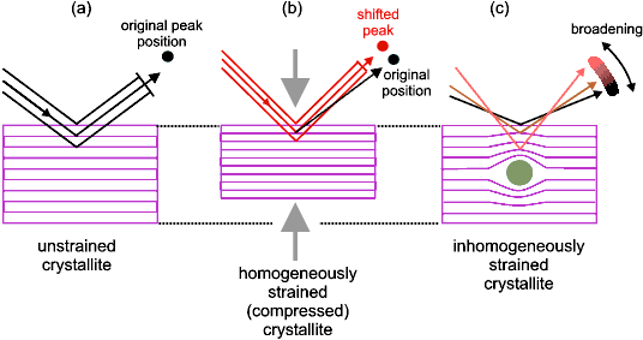
\includegraphics[width=\textwidth]{Stress.png}
            \caption{Crystallite strain}
        \end{figure}
        \vspace{-0.5cm}
        \begin{block}{Strain types}
            \begin{itemize}
                \item Homogeneous: All crystallites were strained equally
                \item Inhomogeneous: Different crystallites are strained by varying amounts
            \end{itemize}
        \end{block}
    \end{columns}
\end{frame}

\begin{frame}{Data visualization}
    \begin{columns}
        \column{0.45\textwidth}
        \onslide<1-> \underline{\textbf{Goal:}} Get linear relationships
        \onslide<2-> \underline{\textbf{Assumption:}} Size and strain broadening are independent
        \onslide<3-> \begin{block}{Change of variables}
            \begin{equation*}
                s = \frac{2 \sin(\theta)}{\lambda}
            \end{equation*}
        \end{block}
        \onslide<4->\begin{exampleblock}{New peak broadening}
            \begin{equation*}
                \delta s = \frac{\cos(\theta)}{\lambda}(\delta 2 \theta)_{corr}
            \end{equation*}
        \end{exampleblock}
        \onslide<5->\begin{block}{Physical constants}
            \begin{itemize}
                \item $D$ : Crystallite size
                \item $e$ : Crystallite strain
            \end{itemize}
        \end{block}
        \column{0.45\textwidth}
        \onslide<6->\begin{alertblock}{Lorentzian broadening}
            \begin{equation*}
                \delta s = \delta(2\theta)_{total} - \delta(2\theta)_{inst}
            \end{equation*}
            \begin{equation*}
                \delta s = \frac{6}{5D} + 2 e s
            \end{equation*}
        \end{alertblock}
        \onslide<7->\begin{alertblock}{Gaussian broadening}
            \begin{equation*}
                [\delta s]^2 = [\delta(2\theta)_{total}]^2 - [\delta(2\theta)_{inst}]^2
            \end{equation*}
            \begin{equation*}
                (\delta s)^2 = \left( \frac{6}{5D} \right)^2 + (2e s)^2
            \end{equation*}
        \end{alertblock}
    \end{columns}
\end{frame}

\begin{frame}{Analysis of \ce{CeO2}}
\vspace{-0.45cm}
    \begin{columns}
        \column{0.5\textwidth}
        \begin{figure}
            \centering
            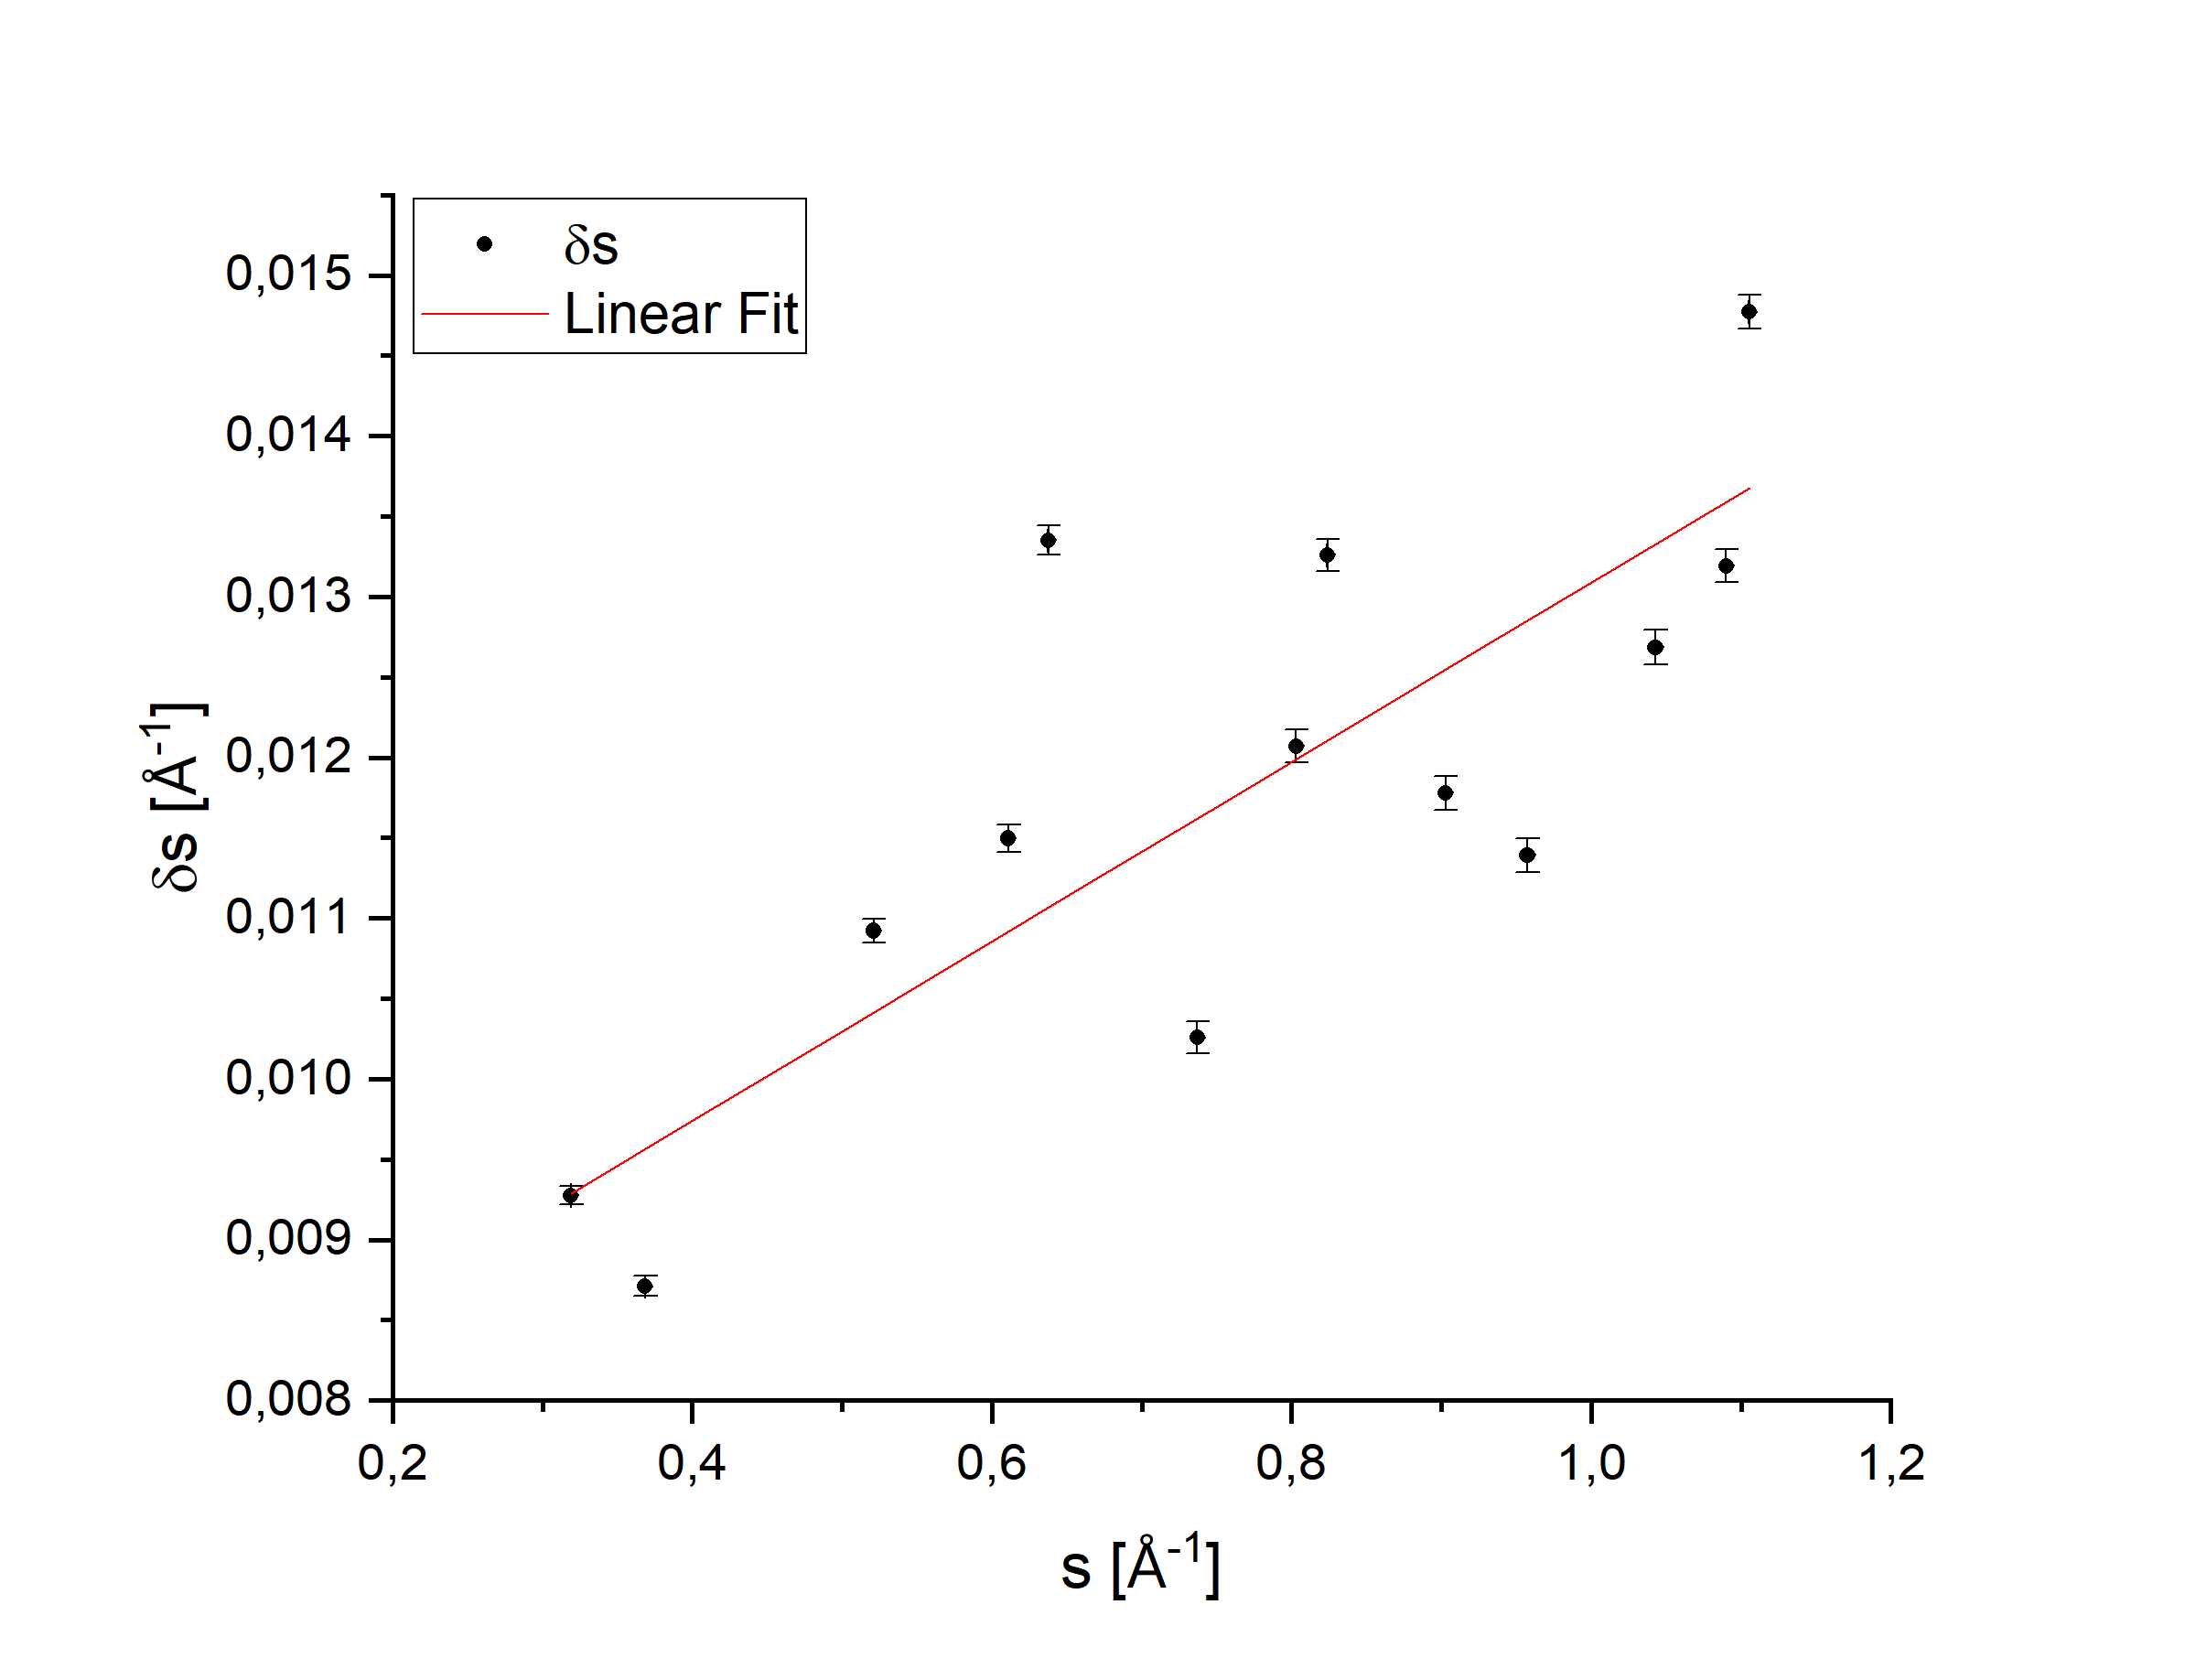
\includegraphics[width=\textwidth]{LorentzianBroadening_CeO2_2.png}
            \caption{Lorentzian approach}
        \end{figure}
        \column{0.5\textwidth}
        \begin{figure}
            \centering
            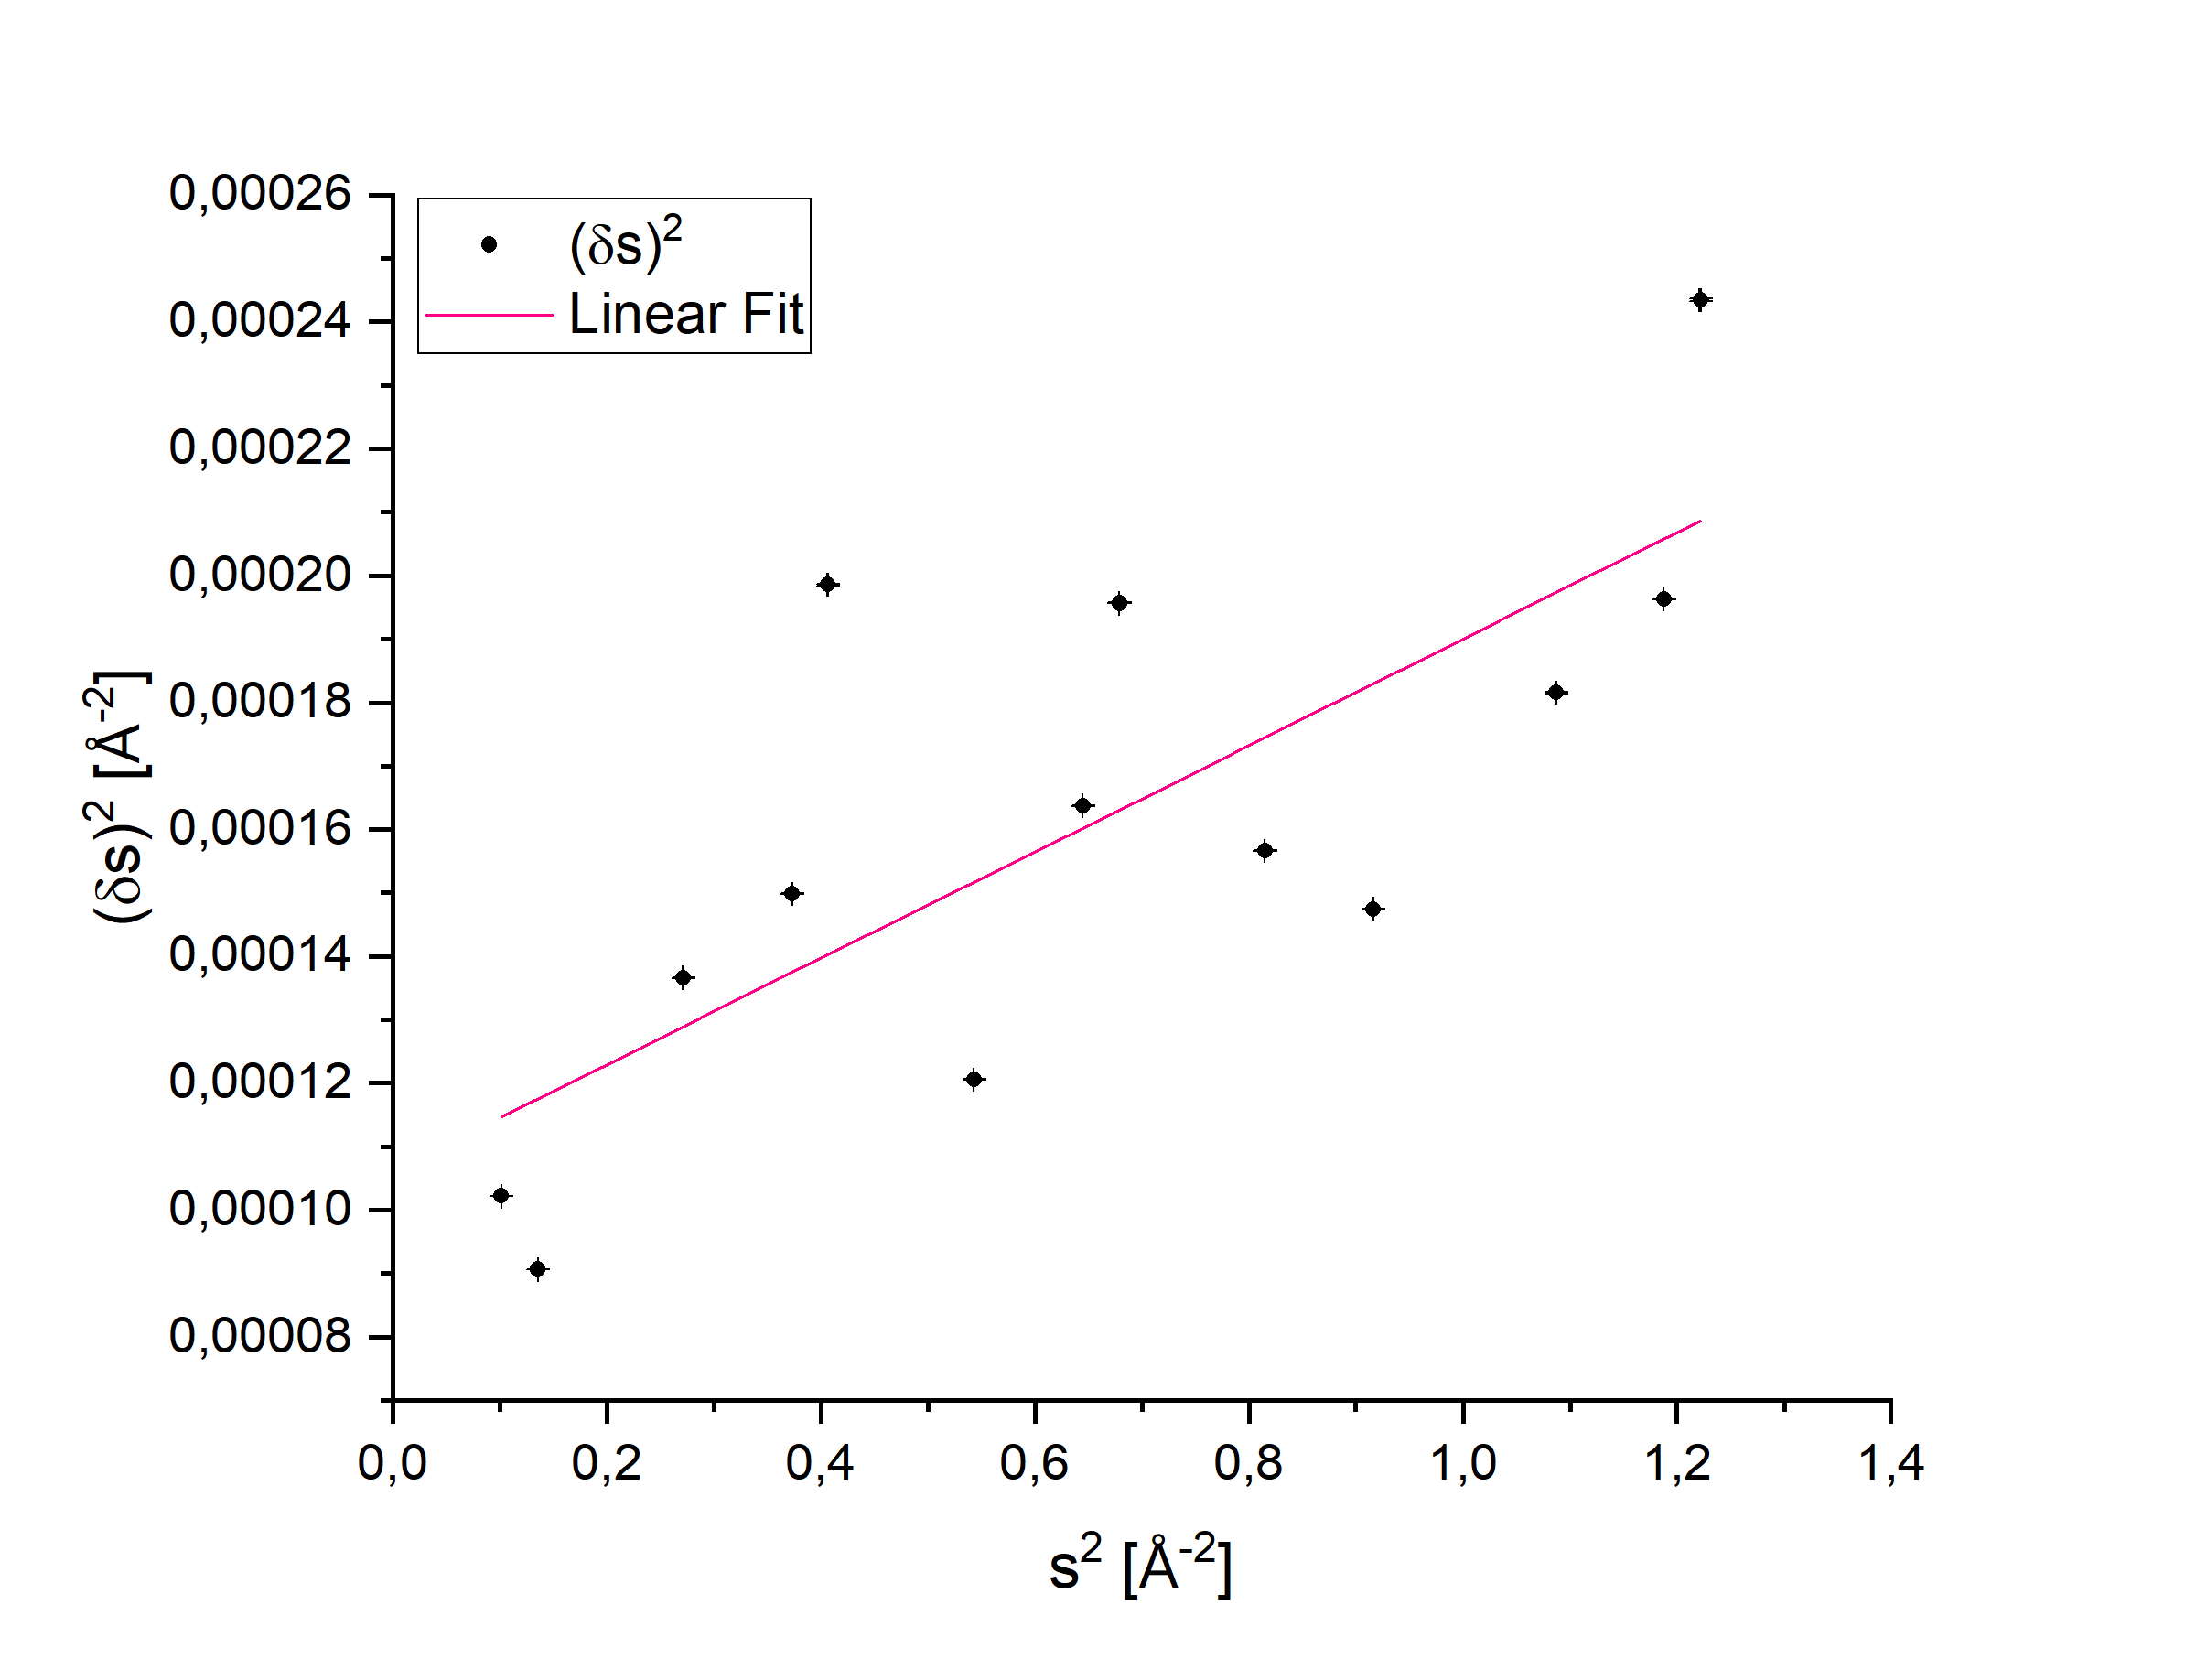
\includegraphics[width=\textwidth]{GaussianBroadening_CeO2_2.png}
            \caption{Gaussian approach}
        \end{figure}
    \end{columns}
    \vspace{-0.5cm}
    \begin{block}{Size and strain}
    \[
        \begin{array}{ll}
            \text{Lorentzian} & \text{Gaussian} \\
             D_L = (15,75 \pm 1,23) \ \si{nm} & D_G = (12,43 \pm 0,98) \ \text{nm} \\
             e_L = (0,27 \pm 0,05) \ \% & e_G = (0,49 \pm 0,05) \ \%
        \end{array}
    \]
    \end{block}
\end{frame}

\begin{frame}{Analysis of \ce{Pd90Au10}}
\vspace{-0.45cm}
    \begin{columns}
        \column{0.5\textwidth}
        \begin{figure}
            \centering
            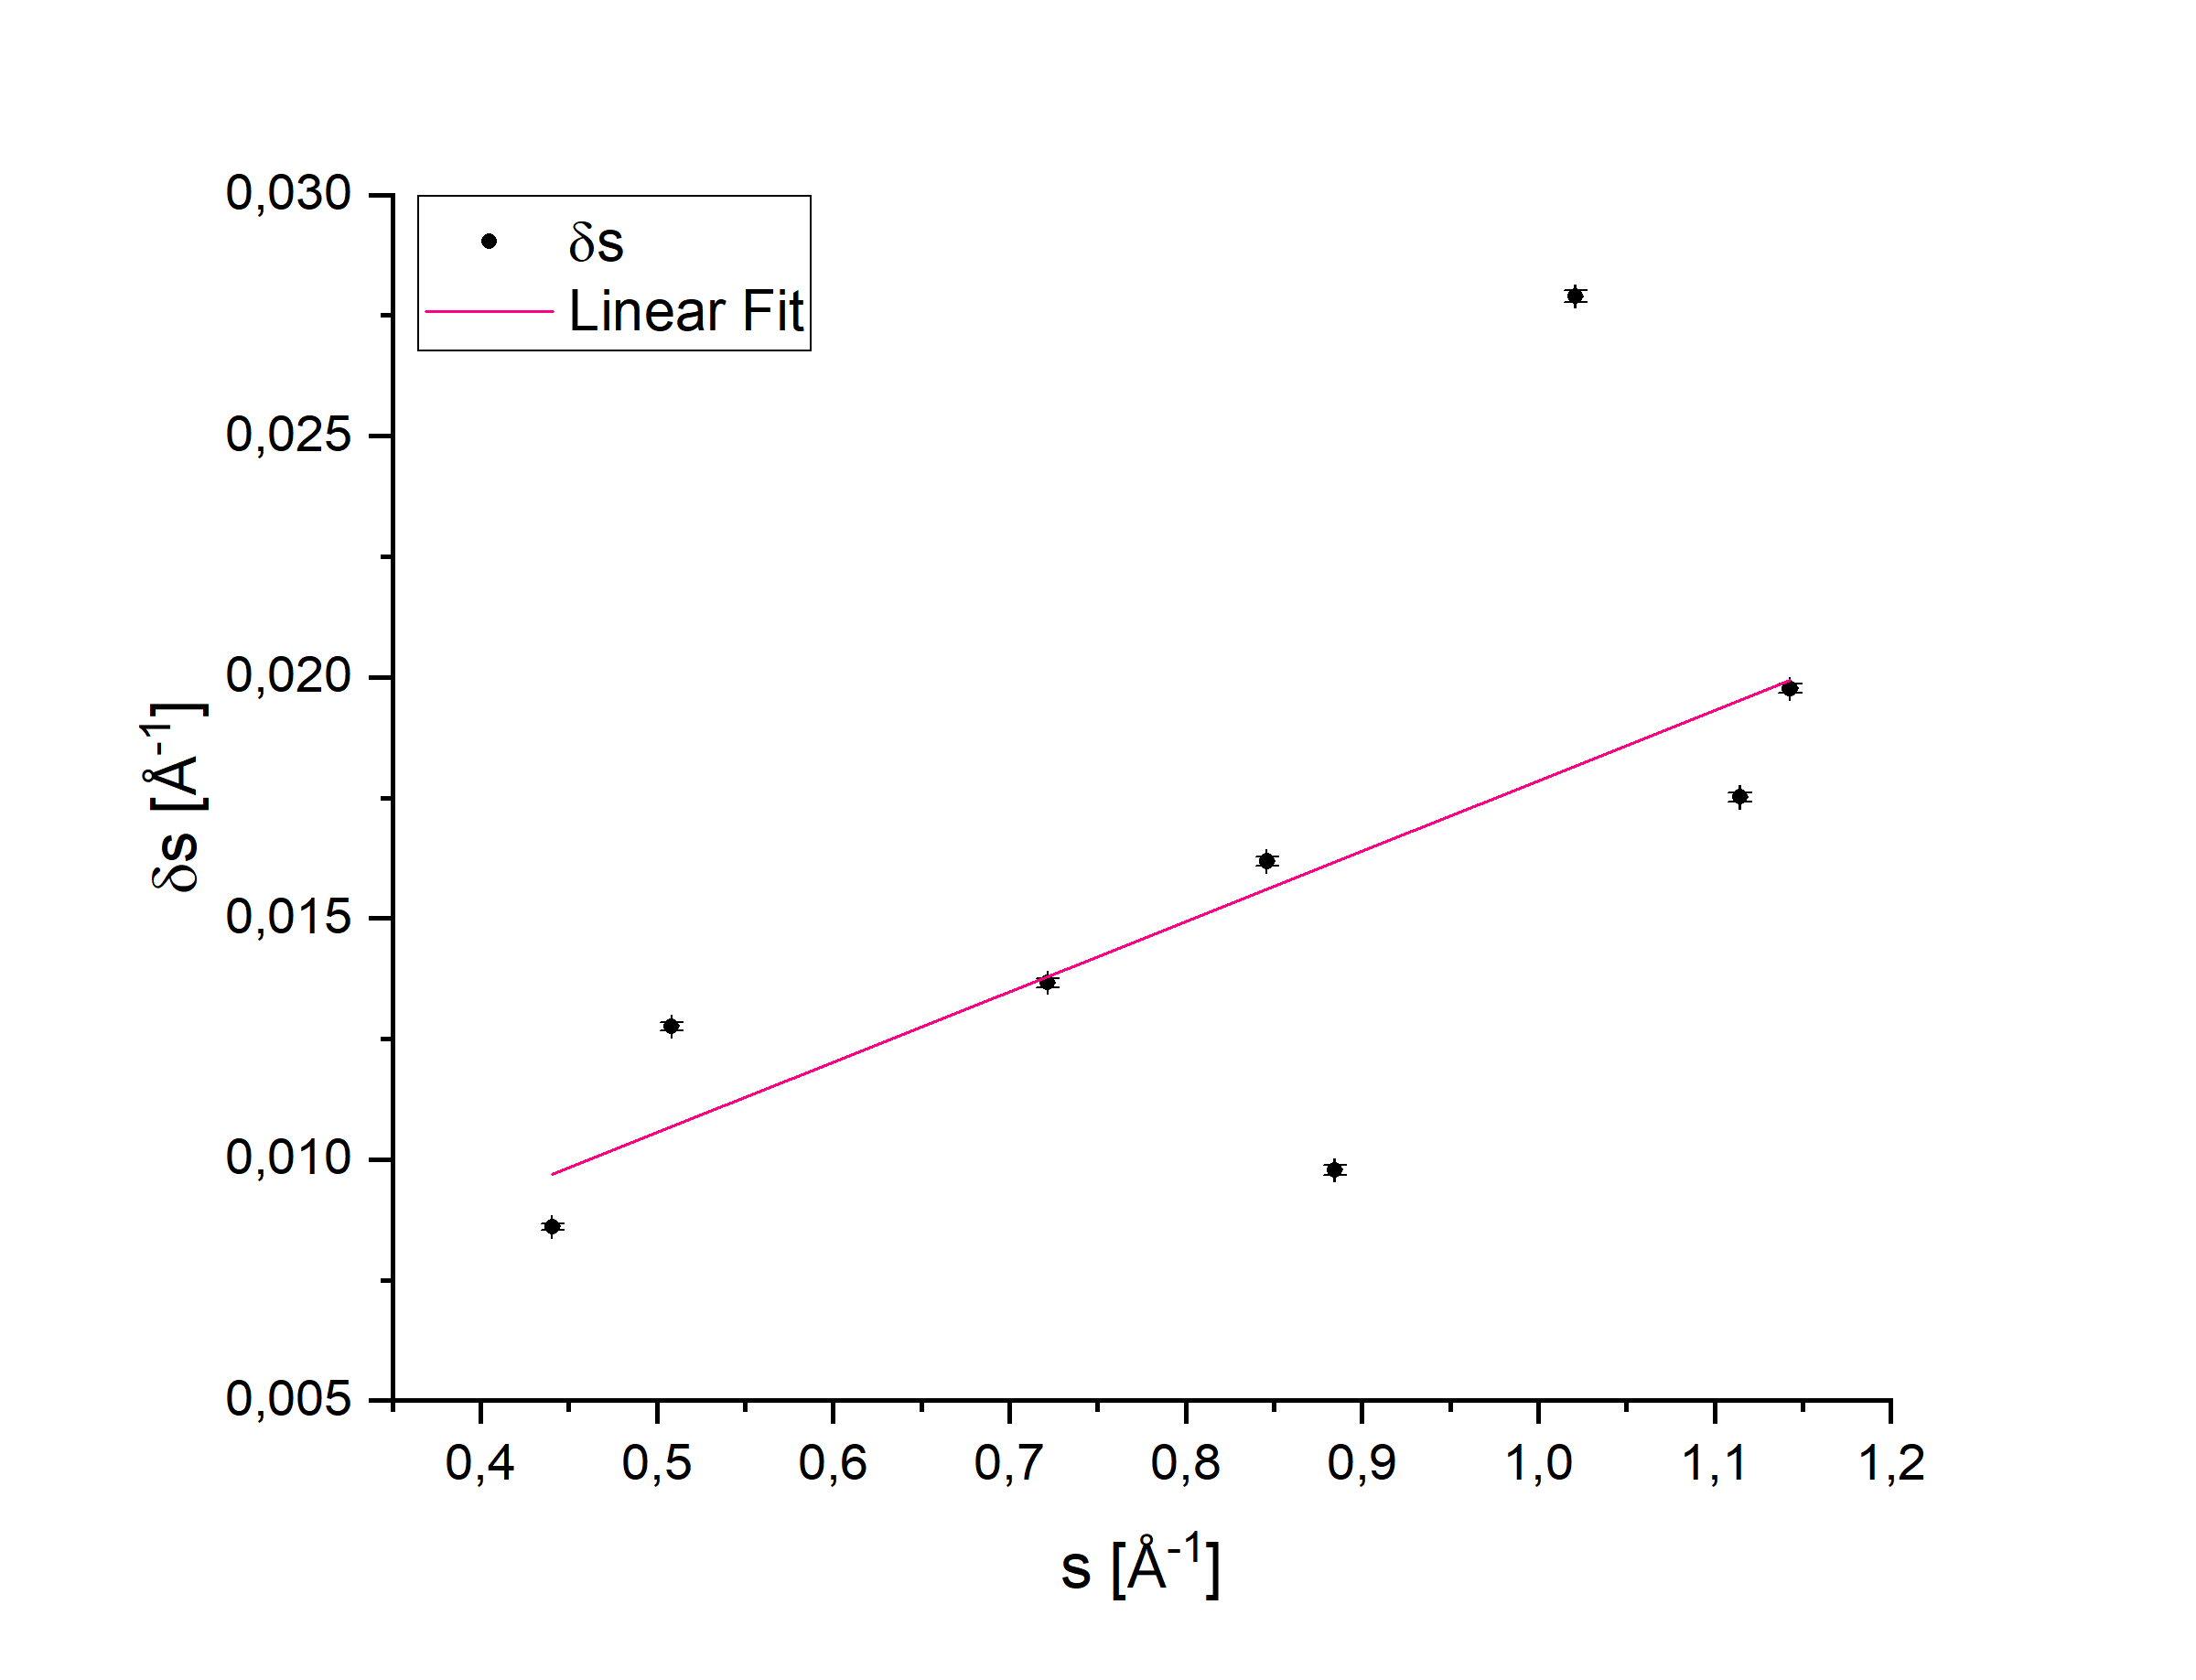
\includegraphics[width=\textwidth]{LorentzianBroadening_Pd90Au10.png}
            \caption{Lorentzian approach}
        \end{figure}
        \column{0.5\textwidth}
        \begin{figure}
            \centering
            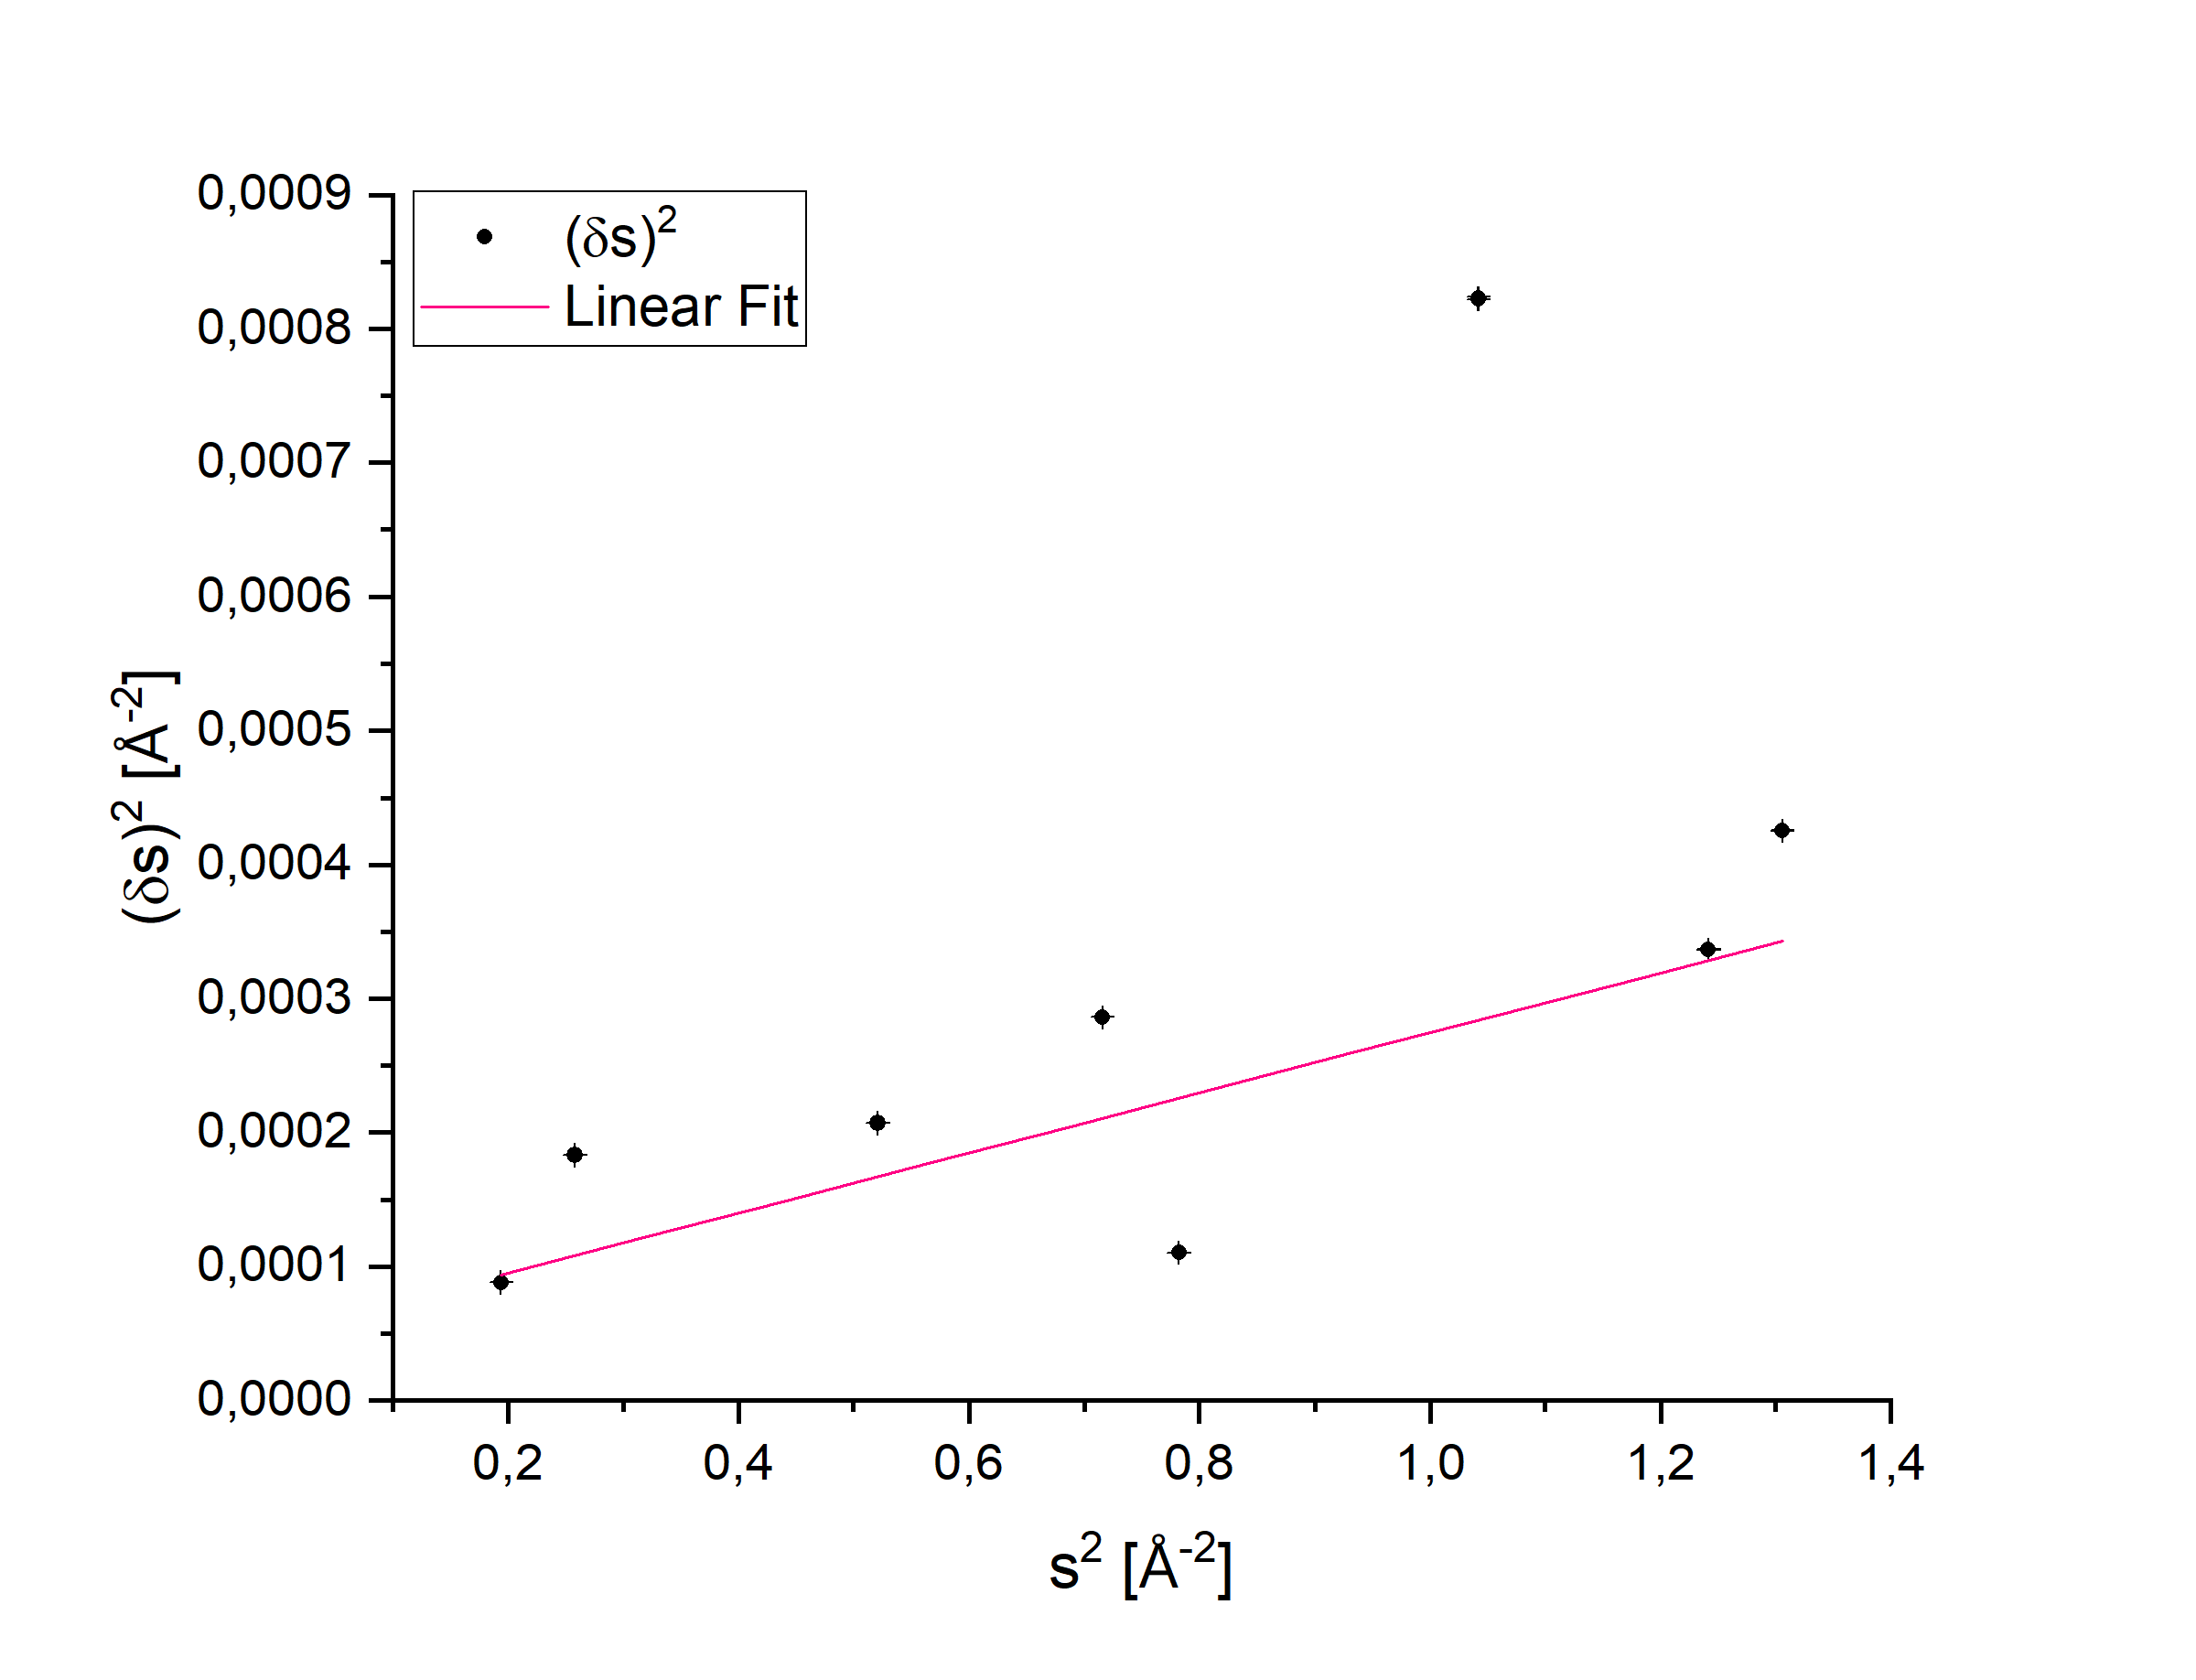
\includegraphics[width=\textwidth]{GaussianBroadening_Pd90Au10.png}
            \caption{Gaussian approach}
        \end{figure}
    \end{columns}
    \vspace{-0.5cm}
    \begin{block}{Size and strain}
    \[
        \begin{array}{ll}
            \text{Lorentzian} & \text{Gaussian} \\
             D_L = (37,15 \pm 24,15) \ \si{nm} & D_G = (16,89 \pm 8,18)\ \si{nm} \\
             e_L = (0,70 \pm 0,16) \ \% & e_G = (0,75 \pm 0,13) \ \%
        \end{array}
    \]
    \end{block}
\end{frame}

\begin{frame}{About the errors}
    \begin{exampleblock}{General error formula}
        $q = f(x_1, \dots, x_n)$
        \begin{equation*}
            \Delta q = \sqrt{ \sum_{i=1}^n \left( \frac{\partial f}{\partial x_i} \Delta x_i \right)^2}
        \end{equation*}
    \end{exampleblock}
    \begin{itemize}
        \item small error bars
        \item scattering of the data points
        \item idealized model, other effects are not considered
    \end{itemize}
\end{frame}

\section{Image References}

\begin{frame}[allowframebreaks]{Image References (in order of appearance)}
    \begin{thebibliography}{50}
    \beamertemplateonlinebibitems
    \bibitem{1}
    X-Ray applications
    \newblock {\em Wikipedia}.
    \newblock \url{https://en.wikipedia.org/wiki/X-ray\#/media/File:X-ray_applications.svg}
    \bibitem{2}
    Water-cooled X-Ray tube
    \newblock {\em Wikipedia}
    \newblock {\url{https://en.wikipedia.org/wiki/X-ray_tube\#/media/File:WaterCooledXrayTube.svg}}
    \bibitem{3}
    Methods for obtaining characteristic Radiation
    \newblock{\em University of Cambridge}
    \newblock{\url{https://www.doitpoms.ac.uk/tlplib/xray-diffraction/production.php}}
    \bibitem{4}
    Bragg Diffraction
    \newblock{\em Wikipedia}
    \newblock{\url{https://en.wikipedia.org/wiki/Bragg's_law\#/media/File:Bragg_diffraction_2.svg}}
    \bibitem{5}
    Face-centered-cubic crystal structure
    \newblock{\em Wikipedia}
    \newblock{\url{https://en.wikipedia.org/wiki/Cubic_crystal_system\#/media/File:Cubic-face-centered.svg}}
    \bibitem{6}
    X-ray Diffraction and Mineral Analysis 
    \newblock{\em Libretexts Geosciences}
    \newblock{\url{https://geo.libretexts.org/Bookshelves/Geology/Mineralogy_\%28Perkins_et_al.\%29/12\%3A_X-ray_Diffraction_and_Mineral_Analysis}}
    \bibitem{7}
    Photocatalytic degradation of pesticides using TiO2 nanoparticles
    \newblock{\em Silpakorn University}
    \newblock{\url{https://www.researchgate.net/publication/294596476_Photocatalytic_degradation_of_pesticides_using_TiO2_nanoparticles}}
    \bibitem{8}
    Basics of X-Ray Powder Diffraction
    \newblock{\em Massachussets Institute of Technology}
    \newblock{\url{http://prism.mit.edu/xray/Basics\%20of\%20X-Ray\%20Powder\%20Diffraction.pdf}}
    \bibitem{9}
    Powder Diffraction
    \newblock{\em University of Cambridge}
    \newblock{\url{https://www.doitpoms.ac.uk/tlplib/xray-diffraction/powder.php}}
    \end{thebibliography}
\end{frame}

\section{Bonus: Vegard law}

\begin{frame}{Vegard law}
    \begin{block}{}
        Element $X$ and element $Y$ in proportions:
        \begin{equation*}
            x:(1-x)
        \end{equation*}
        Lattice constants: $a_X$, $a_Y$
    \end{block}
    \begin{alertblock}{Vegard law}
        \begin{equation*}
            a_{XY} = x \cdot a_X + (1-x) \cdot a_Y  
        \end{equation*}
    \end{alertblock}
    \begin{exampleblock}{\ce{Pd90Au10}}
        $a_{Pd} = 3,859 \ \si{\angstrom} $; $a_{Au} = 4,065 \ \si{\angstrom}$
        \begin{equation*}
            \Rightarrow a_{\ce{Pd90Au10}} \approx 3,88 \ \si{\angstrom}
        \end{equation*}
    \end{exampleblock}
\end{frame}

\end{document}
